%% 
%% Copyright 2007-2020 Elsevier Ltd
%% 
%% This file is part of the 'Elsarticle Bundle'.
%% ---------------------------------------------
%% 
%% It may be distributed under the conditions of the LaTeX Project Public
%% License, either version 1.2 of this license or (at your option) any
%% later version.  The latest version of this license is in
%%    http://www.latex-project.org/lppl.txt
%% and version 1.2 or later is part of all distributions of LaTeX
%% version 1999/12/01 or later.
%% 
%% The list of all files belonging to the 'Elsarticle Bundle' is
%% given in the file `manifest.txt'.
%% 
%% Template article for Elsevier's document class `elsarticle'
%% with harvard style bibliographic references

% == DOUBLE SPACED ==
%\documentclass[review,12pt,authoryear]{elsarticle}
% == SINGLE SPACED ==
\documentclass[12pt,authoryear]{elsarticle}
%\documentclass[final,5p,times,authoryear]{elsarticle}
\usepackage{perpage}
\MakePerPage{footnote}

%% Use the option review to obtain double line spacing
%% \documentclass[authoryear,preprint,review,12pt]{elsarticle}

%% Use the options 1p,twocolumn; 3p; 3p,twocolumn; 5p; or 5p,twocolumn
%% for a journal layout:
%% \documentclass[final,1p,times,authoryear]{elsarticle}
%% \documentclass[final,1p,times,twocolumn,authoryear]{elsarticle}
%% \documentclass[final,3p,times,authoryear]{elsarticle}
%% \documentclass[final,3p,times,twocolumn,authoryear]{elsarticle}
%% \documentclass[final,5p,times,authoryear]{elsarticle}
%% \documentclass[final,5p,times,twocolumn,authoryear]{elsarticle}

%% For including figures, graphicx.sty has been loaded in
%% elsarticle.cls. If you prefer to use the old commands
%% please give \usepackage{epsfig}

%% The amssymb package provides various useful mathematical symbols
\usepackage{amsmath}
\usepackage{amssymb}
\usepackage{mathptmx}
\usepackage{tablefootnote}
\usepackage{geometry}
\usepackage{lineno}
\usepackage{pgfplots}
\usepackage{multirow,tabularx}

% \usetikzlibrary{external}
% \tikzexternalize[prefix=tikz/]

\pgfplotsset{compat=1.17}

\pgfkeys{/pgfplots/.cd,master axis/.style={
    scale only axis,
    enlarge x limits=false,
    axis x line*=bottom,
    xticklabel shift=3pt,
    after end axis/.code={
      \pgfkeys{/pgf/fpu=true,/pgf/fpu/output format=fixed}
      \pgfmathparse{\pgfkeysvalueof{/pgfplots/xmin}}
      \global\let\masterxmin=\pgfmathresult
      \pgfmathparse{\pgfkeysvalueof{/pgfplots/xmax}}
      \global\let\masterxmax=\pgfmathresult
      \pgfkeys{/pgf/fpu=false}
    }
  },
  slave axis/.style={
    scale only axis,enlarge x limits=false,
    axis x line*=top,
    axis y line=none,
    xmin=\masterxmin,xmax=\masterxmax,ymin=0,ymax=1,
    scaled x ticks=false,
    xtick={0,56.020227/ln((2.8-2.7)/(2.8-1.8))*ln((2.8-2.0)/(2.8-1.8)),56.020227/ln((2.8-2.7)/(2.8-1.8))*ln((2.8-2.2)/(2.8-1.8)),56.020227/ln((2.8-2.7)/(2.8-1.8))*ln((2.8-2.4)/(2.8-1.8)),56.020227/ln((2.8-2.7)/(2.8-1.8))*ln((2.8-2.6)/(2.8-1.8)),56.020227/ln((2.8-2.7)/(2.8-1.8))*ln((2.8-2.7)/(2.8-1.8))},
    xticklabel={
      \pgfkeys{/pgf/fpu}
      \pgfmathparse{2.8-(2.8-1.8)*exp(-\tick/(-56.020227/ln((2.8-2.7)/(2.8-1.8))}
      \pgfmathprintnumber{\pgfmathresult}
    }
  }
}

\definecolor{tab_blue}{rgb}{0.1216, 0.4667, 0.7059}
\definecolor{tab_orange}{rgb}{1.0000, 0.4980, 0.0549}
\definecolor{tab_grey}{rgb}{0.4980, 0.4980, 0.4980}
\definecolor{tab_red}{rgb}{0.8392, 0.1529, 0.1569}
\definecolor{tab_brown}{rgb}{0.5490, 0.3373, 0.2941}
\definecolor{tab_purple}{rgb}{0.5804, 0.4039, 0.7412}

\geometry{letterpaper, margin=1in}

\usepackage{xr}
\makeatletter
\newcommand*{\addFileDependency}[1]{% argument=file name and extension
  \typeout{(#1)}% latexmk will find this if $recorder=0 (however, in that case, it will ignore #1 if it is a .aux or .pdf file etc and it exists! if it doesn't exist, it will appear in the list of dependents regardless)
  \@addtofilelist{#1}% if you want it to appear in \listfiles, not really necessary and latexmk doesn't use this
  \IfFileExists{#1}{}{\typeout{No file #1.}}% latexmk will find this message if #1 doesn't exist (yet)
}
\makeatother

\newcommand*{\myexternaldocument}[1]{%
    \externaldocument{#1}%
    \addFileDependency{#1.tex}%
    \addFileDependency{#1.aux}%
}

\myexternaldocument{supplemental}

\graphicspath{{images/}}
%% The amsthm package provides extended theorem environments
%% \usepackage{amsthm}

%% The lineno packages adds line numbers. Start line numbering with
%% \begin{linenumbers}, end it with \end{linenumbers}. Or switch it on
%% for the whole article with \linenumbers.
%% \usepackage{lineno}

\journal{Journal of Aerosol Science}

\begin{document}
%% Left-align equations:
%% \setlength{\mathindent}{0cm}
\begin{frontmatter}

%% Title, authors and addresses

%% use the tnoteref command within \title for footnotes;
%% use the tnotetext command for theassociated footnote;
%% use the fnref command within \author or \affiliation for footnotes;
%% use the fntext command for theassociated footnote;
%% use the corref command within \author for corresponding author footnotes;
%% use the cortext command for theassociated footnote;
%% use the ead command for the email address,
%% and the form \ead[url] for the home page:
%% \title{Title\tnoteref{label1}}
%% \tnotetext[label1]{}
%% \author{Name\corref{cor1}\fnref{label2}}
%% \ead{email address}
%% \ead[url]{home page}
%% \fntext[label2]{}
%% \cortext[cor1]{}
%% \affiliation{organization={},
%%            addressline={}, 
%%            city={},
%%            postcode={}, 
%%            state={},
%%            country={}}
%% \fntext[label3]{}

\title{Differences and similarities in optical properties of coated fractal soot and its surrogates}

%% use optional labels to link authors explicitly to addresses:
%% \author[label1,label2]{}
%% \affiliation[label1]{organization={},
%%             addressline={},
%%             city={},
%%             postcode={},
%%             state={},
%%             country={}}
%%
%% \affiliation[label2]{organization={},
%%             addressline={},
%%             city={},
%%             postcode={},
%%             state={},
%%             country={}}

\affiliation[inst2]{organization={Department of Chemistry and Environmental Science, New Jersey Institute of Technology},%Department and Organization
            city={Newark},
            postcode={07102}, 
            state={New Jersey},
            country={United States}}

\affiliation[inst1]{organization={Department of Chemical and Materials Engineering, New Jersey Institute of Technology},%Department and Organization
            city={Newark},
            postcode={07102}, 
            state={New Jersey},
            country={United States}}

\affiliation[inst3]{organization={Chemical Engineering Department, University of New Haven},%Department and Organization
            city={West Haven},
            postcode={06516}, 
            state={Connecticut},
            country={United States}}


\affiliation[inst4]{organization={Now at: Center for Devices and Radiological Health, Food and Drug Administration},
            state={Maryland},
            country={United States}}

\affiliation[inst5]{organization={Now at: Brookhaven National Laboratory},
            city={Upton},
            postcode={11973}, 
            state={New York},
            country={United States}}

\author[inst2]{Egor V. Demidov}
\author[inst1,inst5]{Ogochukwu Y. Enekwizu}
\author[inst2,inst4]{Ali Hasani}
\author[inst3]{Chong Qiu}
\author[inst2,inst1]{Alexei F. Khalizov}

\begin{abstract}
Atmospheric soot (or black carbon, BC) affects climate through solar light absorption and scattering, which depend strongly on the particle morphology and composition. Initially, soot particles are fractal aggregates of spherules made of  elemental carbon (EC), but condensation of atmospheric trace vapors adds non-EC materials and often results in particle compaction. The optical properties of such processed soot differ from those of fractal soot, and the changes are caused both by particle volume increase from coating addition and by restructuring of the EC backbone. In laboratory studies of soot optics, surrogates such as carbon black (CB) and nigrosin are often used in place of flame-generated soot. Our goal was to investigate if compositional and morphological differences between these surrogates and soot may produce different processing rates and optical responses. In our experiments, we generated fractal soot, compact CB, agglomerated CB (via coagulation of compact CB), and spherical nigrosin aerosol particles, subjected them to supersaturated vapor of dioctyl sebacate (DOS) to form a coating layer, and investigated the morphological response of these four particle types to coating addition and removal. Using coated and coated-denuded aerosol particles with known composition and morphology, we quantified the contributions of volume increase and restructuring to light scattering and absorption enhancements. By comparing experimental measurements against different particle optics models we show that it is crucial to account for larger, multiply charged particles present in the mobility-classified aerosol. Producing a disproportionately high contribution to absolute values of optical cross sections, such larger particles also result in lesser optical enhancements due to slower growth by vapor condensation. Scattering increases for all particle types due to the addition of a coating layer, and also due to restructuring for fractal soot (strongly) and agglomerated CB (weakly). Absorption increases only due to lensing caused by the coating layer for all particle types. We find that simple optical models, such as Mie, are often sufficient to provide reasonable closure with experimental results for bare and coated aerosols, but only after accounting for the contributions from multiply charged particles, both in terms of their stronger optical cross sections and slower condensational growth. We conclude that CB is an appropriate surrogate for soot in aerosol aging studies where the effects of restructuring do not need to be considered and that nigrosin can be used as a general model for light-absorbing aerosols but is not representative of optical properties of soot.
\end{abstract}

%%Research highlights
% \begin{highlights}
% \item Carbon black is an appropriate surrogate for heavily aged soot particles
% \item Nigrosin is not representative of soot but can represent light-absorbing aerosols
% \item Mie provides reasonable closure after accounting for multiply charged particles
% \item Multiply charged particles increase absolute cross-sections but reduce enhancements
% \item Carbon black particles can be generated in compact and semi-fractal forms
% \item Light absorption by fractal soot increases only due to lensing caused by coating 
% \item Light scattering by fractal soot increases due to lensing and restructuring
% \end{highlights}

\begin{keyword}
aerosol \sep soot \sep black carbon \sep carbon black \sep nigrosin \sep aerosol aging \sep light absorption \sep light scattering 
% %% keywords here, in the form: keyword \sep keyword
% keyword one \sep keyword two
% %% PACS codes here, in the form: \PACS code \sep code
% \PACS 0000 \sep 1111
% %% MSC codes here, in the form: \MSC code \sep code
% %% or \MSC[2008] code \sep code (2000 is the default)
% \MSC 0000 \sep 1111
\end{keyword}

\end{frontmatter}

\renewcommand{\thefootnote}{\textit{\alph{footnote}}}

%% \linenumbers
%\linenumbers
%% main text
%% For citations use: 
%%       \citet{<label>} ==> Jones et al. (2015)
%%       \citep{<label>} ==> (Jones et al., 2015)

\section*{Nomenclature}
\begin{tabular}{r c l}
    $m$ & $\rm fg$ & mass of a particle\\
    $D$ & $\rm nm$ & electrical mobility diameter of a particle\\
    $D_{ve}$ & $\rm nm$ & volume-equivalent diameter of a particle\\
    $\rho$ & $\rm g/cm^3$ & material mass density\\
    $V$ & $\rm cm^3$ & volume\\
    $b$ & $\rm Mm^{-1}$ & optical coefficient\\
    $C$ & $\rm \mu m^2$ & optical cross section\\
    $N$ & $\rm 1/cm^3$ & aerosol number density\\
    $N_s$ & $1$ & number of primary particles in a fractal aggregate\\
    $k_0$ & $1$ & fractal pre-exponential factor\\
    $D_f$ & $1$ & fractal dimension\\
    $R_s$ & $\rm nm$ & radius of gyration\\
    $d_p$ & $\rm nm$ & diameter of a primary particle in a fractal aggregate\\
    $\Delta r_{ve}$ & $\rm nm$ & volume-equivalent coating thickness\\
    $\Delta r_m$ & $\rm nm$& coating thickness of a primary particle\\
    $GF_{d}$ & $1$ & electrical mobility diameter growth factor\\
    $GF_{m}$ & $1$ & mass growth factor\\
    $f_i$ & $1$ & relative contribution of mode $i$ to the optical cross section, number fraction\\
    % $\square_0$ & property of a bare particle (subscript)\\
\end{tabular}


\section{Introduction}
Atmospheric aerosols affect climate indirectly by changing cloud properties \citep{lohmann2005global,tao2012impact} and directly by scattering and absorbing sunlight \citep{chylek1995effect}. Among many types of aerosols, soot (or black carbon) is of particular interest, as it strongly absorbs light, thus contributing to global warming, as much as one-third of the contribution of CO\textsubscript{2} \citep{RN21}. Moreover, in many locations worldwide, including major megacities, direct solar heating caused by soot aerosols is comparable with the heating due to greenhouse gases \citep{RN45}. Soot particles suspended in the atmosphere are subject to continuous aging, which changes their microphysical and optical properties, and thus their climatic impacts. Condensation is one of the major aging mechanisms of soot \citep{saathoff2003coating}, and it has been extensively studied using experimental and modeling approaches, including the effects of negative surface curvature \citep{RN70,ivanova2020kinetic} and carbon structure \citep{ivanova2022molecular} on the localization of condensate.

% \textcolor{red}{Ivanova (2022): https://doi.org/10.1021/acs.jced.2c00063}

% \textcolor{red}{Ivanova (2020): https://doi.org/10.1080/02786826.2020.1846677}

% \textcolor{red}{Chen (2018): https://doi.org/10.1021/acs.est.8b04201}

%\citep{RN7,RN4}  \citep{RN51,mikheev2002laboratory}. 


% \textcolor{red}{Zangmeister (2009), Khalizov (2009), Ma (2013), and Mikheev (2002) are not appropriate references} 

Soot particles are fractal aggregates of graphitic primary spherules and their principal source is the incomplete combustion of carbonaceous matter. Combustion can be used to generate soot aerosols in the laboratory to study their transformations and properties. However, since particle size, organic carbon content, morphology, and concentration of flame-generated soot are highly sensitive to combustion and sampling conditions \citep{RN46,RN47}, researchers often prefer to use pre-made products instead, like carbon black (CB). Such products are manufactured industrially to serve as ink pigments, material additives, etc., making them inexpensive and readily available \citep{RN12}. In spite of a different name, carbon black is inherently the same material as soot. The combustion conditions for CB are much more well controlled to leading to less variability in the generated products. The key difference between CB and flame-generated soot is that the former can be distributed in the form of an aqueous suspension, where aggregates are present as near-spherical particles. In contrast, soot generated and sampled in a flame retains its fractal morphology until the controlled aging process is deliberately initiated, allowing to evaluate changes in optical properties that are induced by not only a coating layer addition, but also by restructuring of the particles.

Advantages of using CB in place of soot include high carbon content, stable number density and size distribution, constant morphology and composition, ease of generation, and safety, as generation does not involve flames. Indeed, a simple atomizer that nebulizes a suspension of carbon black particles can generate a stable output over extended time. "Cab-O-Jet" (a brand CB) has been used in a number of studies, including an intercomparison of aerosol absorption cross sections measured with photoacoustic spectroscopy \citep{RN3}, the size and wavelength dependence of optical properties of bare particles \citep{RN4}, and also a comparison of mass absorption spectra obtained at different labs against other surrogates, such as graphene nanoplatelets and fullerene soot \citep{RN63}. These studies concluded that measurements reported by different labs were generally consistent and that surrogates are suitable for instrumental intercomparison. That would likely not be the case with the flame-generated soot, because slight variations in combustion conditions can lead to drastic differences in particle morphology and composition \citep{moore2014mapping}, and hence optics. Another brand of CB, "Regal Black" \citep{RN65}, was used as proxy for collapsed soot to study the response of a Single-Particle Soot Photometer (SP2) to morphology of composite particles produced by coagulation of light absorbing and non-absorbing aerosols, including sodium chloride, ammonium sulfate, and dioctyl sebacate.

Some researchers go as far as to use nigrosin as a surrogate for absorbing aerosols \citep{RN8,RN54,RN55,RN56,RN57,drinovec2022dual}. Nigrosin is a water-soluble organic dye for negative staining of bacteria, which can be nebulized from its solution, and when droplets evaporate upon mixing with dry air, spherical particles are formed. Since nigrosin particles are not fractal, they lack the ability to restructure. Also, being solid spheres, nigrosin particles lack interstitial space that can be present in CB and compacted soot. One factor making nigrosin an attractive surrogate is that extinction and scattering cross sections can be easily calculated for its spherical particles, presumably making experimental results easy to verify computationally. However, when particles are size classified based on their electrical mobility, the resulting aerosol is not truly monodisperse, containing a fraction of multiply charged particles of larger sizes \citep{mcmurry2002relationship,pagels2009processing}. These larger particles have significantly higher absorption and scattering cross-sections, which can bias high optical measurements \citep{RN50} and cause a significant deviation from theoretical predictions. There are ways to account for the presence of multiply-charged particles for both bare and coated aerosols \citep{RN67, RN77}, but the procedures are not always trivial and additional measurements are often required.

This study explores experimentally how flame-generated soot aggregates and their surrogates (commercial CB and nigrosin) respond morphologically and optically to coating by a low-volatility organic compound, dioctyl sebacate (DOS). For CB, we report measurements for both compact aggregates and agglomerates of compact aggregates. Corrections for multiple charging are applied and their efficacy is analyzed and discussed for different particle types. Finally, the optical properties of soot, two forms of CB, and nigrosin are compared against each other and also against three commonly used optical models, to determine applicability ranges for the optical models and soot surrogates.


\section{Methodology}


The system used to generate and process aerosols is illustrated in Figure \ref{fig:system}. It comprised an aerosol generation unit (either an atomizer or an inverted diffusion flame burner), a differential mobility analyzer (DMA, TSI Model 3081A) with home-built recirculating sheath flow and high voltage control to produce electrical mobility-classified aerosol, a temperature-controlled coating chamber, a thermal denuder to remove coating from aerosol \citep{RN39}, an aerosol particle mass analyzer (APM, Kanomax Model 3601) to measure mass of aerosol particles, a second DMA to measure electrical mobility diameter of aerosol particles processed by coating or coating followed by denuding, a cavity attenuated phase shift spectrometer (CAPS PM\textsubscript{SSA}, Aerodyne Research, 525 nm wavelength) to measure aerosol extinction and scattering coefficients, and a condensation particle counter (CPC, TSI Model 3772) to measure aerosol particle number density. The components of the system were connected with stainless steel tubing segments joined together with conductive silicone tubing. The entire system was conrolled by LabView codes, and a detailed description of the system and its individual components can be found in our previous work \citep{RN48,RN49}.

\begin{figure}[ht]
\centering
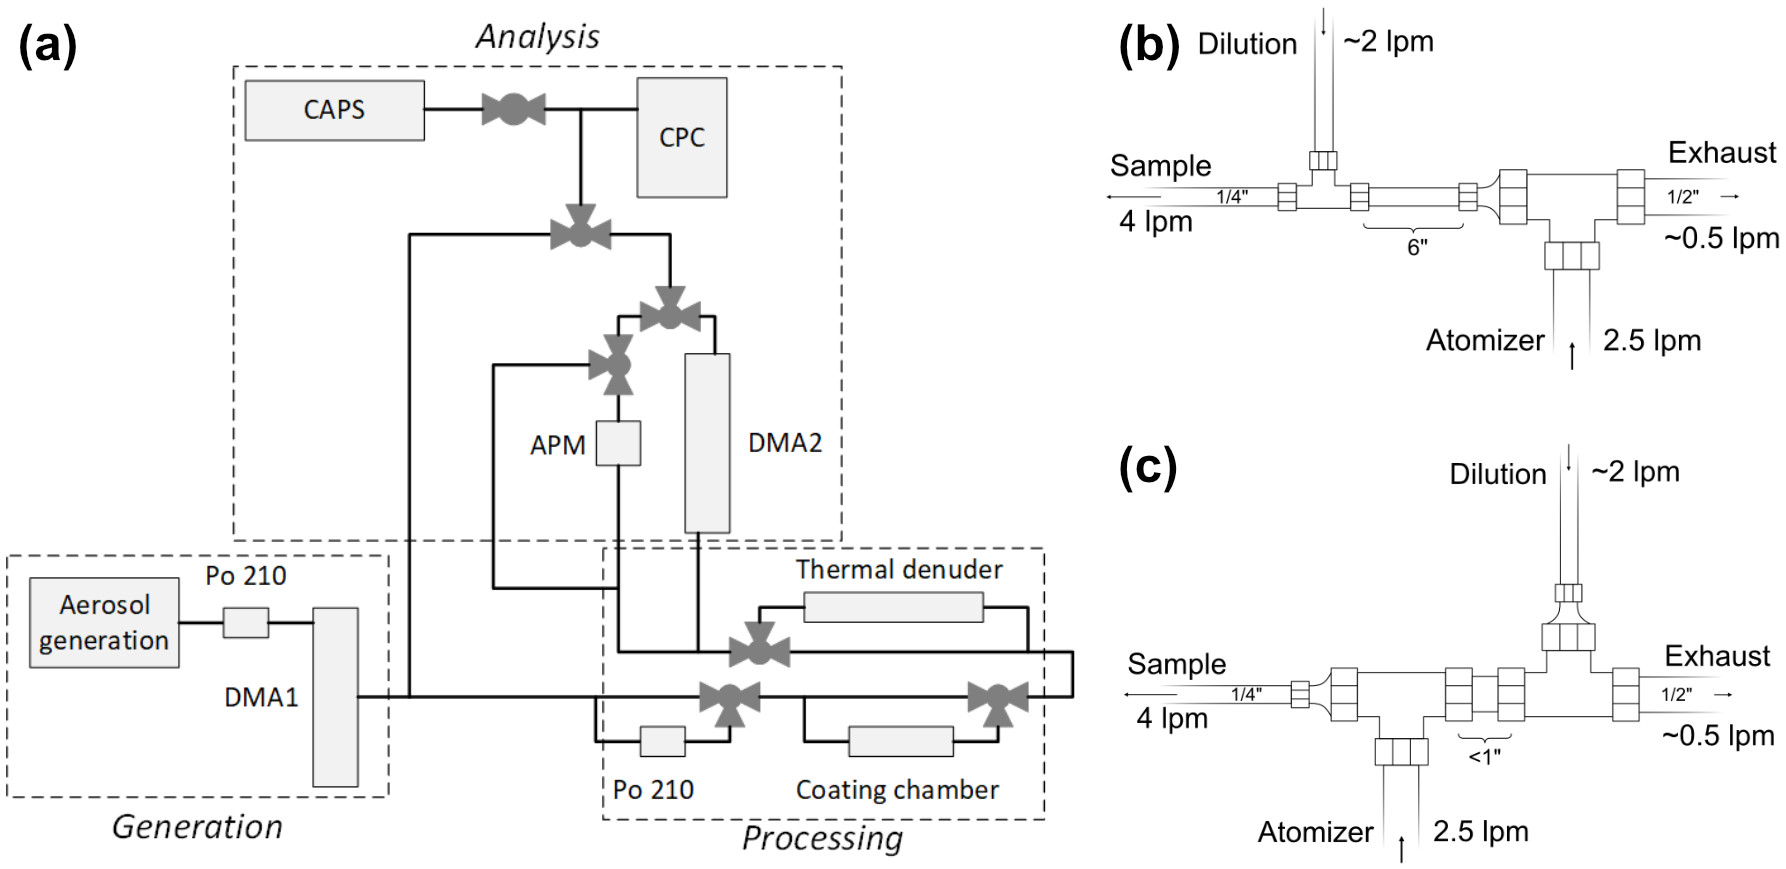
\includegraphics[scale=0.7]{system_diagram.png}
\caption{Aerosol generation and processing system}
\label{fig:system}
\end{figure}

\subsection{Particle generation and processing}

Soot was generated by incomplete combustion of natural gas in an inverted diffusion flame burner \citep{RN43,RN44} and sampled using an ejector dilutor. Carbon black suspension (Cab-O-Jet 200, Cabot Corporation) and nigrosin solution (Nigrosin water soluble, Alfa Aesar) were prepared with distilled water and corresponding aerosols were generated with a constant output atomizer (TSI Model 3076). To generate compact CB, the nebulized aqueous aerosol was immediately diluted with dry air. To generate agglomerated CB, the nebulized aerosol was diluted a few centimeters downstream from the atomizer, which provided sufficient residence time for concentrated aerosol droplets to coagulate, producing agglomerated CB particles after drying. In some experiments, polystyrene latex (PSL) aerosols of different particle sizes were generated from suspensions of nanospheres (3000 Series Nanosphere, Thermo Scientific). The aerosols were brought to quilibrium charge distribution with a bipolar \textsuperscript{210}Po charger (Staticmaster Static Eliminator, 500 µCi) and size-classified with DMA1. It is important to note that particles carrying multiple charges behave as if they were smaller in an electric field of the DMA. Therefore, aerosol after DMA1 is pseudo-monodisperse.

The size-classified aerosol was coated by passing it through a temperature-controlled coating chamber, which is a cylindrical borosilicate glass container (45 cm length and 2 cm inner diameter) partially filled with dioctyl sebacate and wrapped in heating tape and insulation. DOS was selected as the coating material because of its low volatility (saturated vapor pressure of $9.69\times10^{-6}\ \mathrm{Pa}$ at $25\ \mathrm{^{\circ}C}$) and frequent use to study soot processing and optics.
%\textcolor{red}{Do we need the following sentence here? [The refractive index of DOS (1.43+0i) is in the range of refractive indices of many liquid coating materials \citep{RN22}]}. 
Adjusting the temperature of the coating chamber allowed the control of DOS condensation on particles. In some experiments, the condensed coating material was subsequently removed from particles by passing them through a thermal denuder operated at 300 °C. All particles were passed through an identical denuder prior to aging to ensure that any optical response of coated-denuded particles was not induced by the high temperature in the denuder. Particle mass and electrical mobility diameter of processed aerosol were measured by sending the flow through the APM and DMA2, respectively. Both DMAs were operated at a sheath-to-sample flow ratio of 6.5, using sample and sheath flows of 1.0 and 6.5 liters per minute (lpm). The APM operated at a sample flow of 0.3 lpm, which was achieved by removing 0.7 lpm before the APM and then adding 0.7 lpm of filtered clean air after the APM, using volumetric flow controllers connected to a vacuum pump and pressurized air, respectively.

Mass measurements were used to determine the amount of coating condensed and electrical mobility diameter was used to quantify the extent of restructuring. Mass of processed particles, $m$ was normalized by mass of fresh particles $m_0$ to obtain the mass growth factor.
\begin{equation}
\mathrm{Gfm}=\frac{m}{m_0}
\label{eq:gfm}
\end{equation}
Mass growth factor was converted into volume-equivalent coating thickness, $\Delta r_{ve}$, to facilitate the comparison in the amount of coating gained by particles of different initial volume-equivalent diameters \citep{RN37}.
\begin{equation}
\Delta r_{ve}=\frac{1}{2}D_{ve,0}\left(\sqrt[3]{\frac{V}{V_0}}-1\right)=
\frac{1}{2}D_{ve,0}\left(\sqrt[3]{1+\frac{\rho_{\rm core}}{\rho_{\rm shell}}\left(\mathrm{Gfm}-1\right)}-1\right)
\label{eq:drve}
\end{equation}
Where $D_{\rm ve,0}$ is volume-equivalent diameter of a bare particles, $V$ is volume of a coated particle, $V_0$ is volume of a bare particle, $\rho_{\rm core}$ is material density of a bare particle, and $\rho_{\rm shell}$ is density of the coating material.

Similarly, the electrical mobility diameter of processed particles, $D$ was normalized by the electrical mobility diameter of fresh particles, $D_0$, to obtain the electrical mobility diameter growth factor.
\begin{equation}
\mathrm{Gfd}=\frac{D}{D_0}
\label{eq:gfd}
\end{equation}
$\rm Gfd$ was obtained from Tandem DMA (TDMA) scans, where particles were size-classified with DMA1, processed by coating or coating-denuding, and then their size distribution was measured with DMA2.

\subsection{Particle sample collection and imaging}

Samples of size-classified unprocessed aerosol particles were collected on silicon chips, using a custom-built electrostatic precipitator \citep{RN17,RN16} placed after DMA1. In the precipitator, high voltage (3-4 kV) applied to the chip holder created an electric field between the chip and grounded body of the precipitator, causing charged aerosol particles to travel toward and deposit on the silicon chip. After an hour of collection, chips were removed from the precipitator and imaged with a scanning electron microscope (SEM, JEOL JSM-7900F). Before collection, silicon chips were prepared by washing with methanol in an ultrasound bath and drying with nitrogen gas. To quantify particle compactness, convexity was calculated from SEM images as the ratio of the particle projected area ($A_p$) to the area of a convex hull polygon.

\begin{equation}
    \mathrm{Convexity}=\frac{A_p}{A_{polygon}}
    \label{eq:convexity}
\end{equation}

\subsection{Optical measurements}

To measure number density and optical properties of aerosol concurrently, a makeup flow of 0.87 lpm was added and then the sample flow was split iso-kinetically in two separate flows directed to CAPS PM\textsubscript{SSA} (0.87 lpm) and CPC (1.0 lpm), respectively. An orifice inside the valve ensured mixing of the aerosol stream and the dilution air stream. The distances from the split to CAPS PM\textsubscript{SSA} and CPC were adjusted to ensure equal wall losses, so that the particle number density measured by the CPC corresponded to the number density within the CAPS PM\textsubscript{SSA} cell. We found that it was crucial to install a denuder filled with XB-17 (a mixture of activated charcoal and permanganate-impregnated alumina, General Carbon Corp.) after DMA1 during experiments with flame-generated soot to remove traces of NO\textsubscript{2} produced by the burner. NO\textsubscript{2} is a strong light absorber at 525 nm and its concentration is highly sensitive to combustion conditions. In the absence of the denuder, light extinction measurements were subject to significant variability, requiring that baselines to be taken frequently.

The CAPS PM\textsubscript{SSA} measured extinction and scattering coefficients ($b$) of bare and processed aerosol particles. Absorption coefficients were calculated as a difference of extinction and scattering coefficients \citep{RN7,RN50}.
\begin{equation}
b_{\rm abs}=b_{\rm ext}-b_{\rm sca}
\label{eq:babs}
\end{equation}
The coefficients were converted to cross sections ($C$) by normalizing them by aerosol number density ($N$):
\begin{equation}
C=\frac{b}{N}
\label{eq:copt}
\end{equation}

To obtain accurate optical data, scattering and extinction coefficients were recorded every five seconds over three minutes for each measurement. Arithmetic mean of the cross sections acquired over a three-minute interval was calculated and reported as the optical measurement. Baselines were taken prior to each measurement, where aerosol flow was redirected through a filter (United Filtration DIF-BN60) located inside the CAPS PM\textsubscript{SSA} to flush its optics cell and measure extinction and scattering of gas without particles.

\subsection{Numerical aggregate generation for discrete dipole approximation calculations}

Soot aggregates of fractal ($D_f < 2.1$) and compact ($D_f > 2.1$) morphologies were simulated using a cluster-cluster aggregation (CCA) algorithm developed by \citet{RN35}. The CCA method, described here in brief, is based on a hierarchical scheme of aggregation of smaller sub-clusters, which obey the fractal scaling law \citep{jullien1987aggregation},
\begin{equation}
N_s=k_0\left(\frac{2R_s}{d_p}\right)^{D_f}
\label{eq:fractal}
\end{equation}
where $N_s$ is the number of primary particles, $k_0$ is the pre-exponential factor, $R_s$ is the radius of gyration, $d_p$ is the diameter of primary units, and $D_f$ is the fractal dimension. In this context, where all the primary particles are assumed to be of the same size, $R_g$ is defined as the root mean squared distance of primary particles from the center of mass of the aggregate. Equal-sized primary particles are characteristic of many laboratory generated soot aggregates \citep{RN22,RN25}.

Aggregate generation involves sequentially combining smaller sub-aggregates into bigger clusters until the target aggregate size $N$ is reached. Every time two sub-aggregates are combined into a cluster, radius of gyration of the formed cluster, $R_{g,\rm new}$, depends on radii of gyration of its two constituent sub-aggregates, $R_{g,1}$ and $R_{g,2}$, and on how those sub-aggregates are combined. Therefore, $R_{g,\rm new}$ of the formed cluster can be controlled by varying the orientations of the sub-aggregates and the location of the point where they are joined. A function $R_{g,\rm new}(R_{g,1},R_{g,2},D_f,k_0)$ is derived from the fractal scaling law and the definition of $R_g$. Then, at every step where sub-aggregates are combined, $R_{g,\rm new}$ is prescribed by the fractal scaling law and orientations and joining positions are varied randomly until $R_{g,\rm new}$ of the combined cluster is within error tolerance from the target value. Thus, by constraining the way sub-aggregates are combined, an aggregate conforming to Equation \ref{eq:fractal} is generated. Aggregates produced by the CCA algorithm are representative of real soot particles formed via diffusion-limited cluster aggregation \citep{RN36}.

To discretize the aggregate for use with DDA, a three-dimensional Cartesian grid is created and the generated fractal aggregate is placed in this Cartesian space. For each spherical particle comprising the aggregate, grid elements that fall within the boundary of the sphere are filled with black carbon. To add a uniform coating to the discretized aggregate, the function described in \citet{RN22} is used to compute the boundary of the coating layer and all the grid elements that are within the boundary of the coating, but are not already filled with black carbon, are then filled with the coating material.

% The aggregate generation process begins with a set of isolated identical spherical primary particles, $N_M \ge N_s$. A random pair is picked and joined at a random contact point leaving $N_M–1$ primary particles. A new pair is selected from the set and joined. The combination of a pair of clusters is constrained by the distance between the centers of masses of the two clusters, which is such that Equation \eqref{eq:fractal} still holds. The combining clusters are then rotated as solid bodies until they have at least one contact point and no overlapping. After performing the procedure for all clusters on one level, another level involving larger clusters begins and the procedure is repeated till the aggregate attains the desired number of primary particles, $N_s$, which was set to 120, roughly corresponding to fractal soot aggregates of 240 nm mobility diameter used in our experiments. The simulated aggregates are assumed to be monodisperse with a primary particle diameter, $R_s$ set to 28 nm, which is typical for some laboratory generated soot aggregates \citep{RN22,RN25}. To generate coated soot, the coating material was applied to obtain a uniform coating distribution on the bare aggregates as described by \citet{RN22}. Aggregates produced by the CCA algorithms are representative of real soot particles formed via diffusion-limited cluster aggregation \citep{RN36}.

\subsection{Optical models}

Mie theory, Rayleigh-Debye-Gans (RDG),  and discrete dipole approximation (DDA) were used to predict optical properties of bare and coated particles. Mie theory provides a solution for electromagnetic wave scattering and extinction by a sphere \citep{RN1}. A modification of Mie for coated spheres, implemented by \cite{RN19}, was used to model coated particles in this study. Mie provides an exact solution for spherical particles (e.g., nigrosin) and should be in a reasonable agreement with experimental data for compact particles, such CB, thickly coated soot, or coated-denuded soot, due to their near-spherical shape.

The RDG approximation \citep{RN40,kerker2016scattering} can be used to provide a better estimate of optical properties in the case of fractal aggregates. Absorption cross section (Equation \ref{eq:rdg}) of an aggregate is approximated by a product of the absorption cross section of an individual primary particle ($C_\mathrm{abs,monomer}$) and the number of individual primary particles ($N$). In conjunction with core-shell Mie theory, RDG can be used to predict light absorption by thinly coated fractal aggregates (RDG-Mie). We do not consider RDG scattering because it requires the fractal dimension of aggregates, experimental determination of which is beyond the scope of this study. To extend the RDG approach to coated aggregates, the coating material is distributed over the primary particles as spherical shells and absorption cross sections are computed for the coated primary particles using core-shell Mie. Then, absorption cross sections of coated primary particles are scaled to aggregates according to RDG theory.
\begin{equation}
    C_\mathrm{abs,aggregate}=NC_\mathrm{abs,monomer}
    \label{eq:rdg}
\end{equation}
When the diameter of primary particles in an aggregate is known, volume equivalent coating thickness of a primary particle can be related to volume-equivalent coating thickness of the aggregate with Equation \ref{eq:drve_monomer}:
\begin{equation}
    \Delta r_{m}=d_m\frac{\Delta r_{ve}}{D_0}
    \label{eq:drve_monomer}
\end{equation}

DDA \citep{RN33} is a versatile approach for predicting the optical properties of particles of arbitrary geometry that has been used in a large number of soot modeling studies \citep{RN26,RN27,RN28}. In DDA, the particle shape is described as a collection of small discrete volumes (dipoles) that interact with electromagnetic waves and each other. To converge to an accurate solution, the interdipole separation, $d$, has to be chosen sufficiently small such that the quantity $|n|kd < 1$, where $n$ is the complex refractive index and $k = 2\pi/\lambda$ is the wavenumber, with $\lambda$ being the incident wavelength. This is to ensure that the dipole approximation holds \citep{RN29} and that the geometry of the particle is well approximated by an array of dipoles \citep{RN30}.

Optical modeling was performed using the refractive indices shown in Table \ref{tab:refindices}. The refractive index of soot is based on the expression reported by \citet{RN23}. For a wavelength of 530 nm, the refractive index was $1.73+0.6i$, falling within the range recommended by \citet{RN34} for visible light. The refractive index of the organic coating was assumed to be $1.43+0i$ and is representative of many organic materials \citep{crchandbook}, including DOS, which was used in our experiments. By comparing DOS with other chemicals of similar structure, we found that the refractive index varied by less than  $\pm0.03$, causing a $\pm 3.5\%$ variation in scattering and $\pm 2.5\%$ variation in absorption by a 150 nm absorbing sphere with a 20 nm coating. Such variation is within the error range of our experimental measurements.

Optical measurements were conducted at 525 nm wavelength, while DDA calculations were performed for 530 nm wavelength. According to our sensitivity analysis, the difference in scattering is $0.4 \%$ and the difference in absorption is $0.3 \%$ for a 150 nm absorbing sphere with a 20 nm coating at 525 and 530 nm wavelength. This difference is within the error of our experimental measurements, which means that DDA calculations are representative of experimental data.

\begin{table}[ht]
\caption{Refractive indices of materials used in optical calculations}
\label{tab:refindices}
\begin{center}
\begin{tabular}{ l c } 
 \hline
 \multicolumn{1}{c}{Material} & Complex refractive index \\
 \hline
 Soot/carbon black\textsuperscript{\textit{a}} & 1.73+0.60i\\
 Nigrosin\textsuperscript{\textit{b}} & 1.71+0.27i\\
 Liquid organic compounds\textsuperscript{\textit{c}} & 1.43+0.00i\\
 \hline
\end{tabular}
\end{center}

\textsuperscript{\textit{a}}\citet{RN23}\\
\textsuperscript{\textit{b}}\citet{RN15}\\
\textsuperscript{\textit{c}}\citet{RN22}
\end{table}

For this study, the Amsterdam DDA (ADDA) version 1.3 \citep{RN11}, an open-source C implementation of DDA, was used. For each bare or coated soot aggregate, orientation-averaged extinction, scattering, and absorption cross-sections ($C_{\rm ext}$, $C_{\rm sca}$, $C_{\rm abs}$) were determined. The interdipole separation, $d$ was varied from 2 nm down to 0.8 nm, resulting in approximately 1400 to 22,000 dipoles per single monomer volume. The maximum dipole size of 2 nm was only used for thickly coated aggregates (i.e., $\Delta r_{ve}\ge 18\ \rm nm$). Small dipole sizes ensured that both the coating and morphological features were accurately represented i.e., there were no shape approximation errors. Under these circumstances $|m|kd$, was less than 0.1 and satisfied the restriction set by \citet{RN32} for obtaining accurate optical predictions for soot aggregates. The calculated optical properties presented in this study are an average of three aggregate realizations belonging to the same class of fractal parameters ($N_s$, $R_s$, $D_f$, $k_0$). The relative standard deviations (RSD) obtained were less than $1\%$.


\section{Results and discussion}
\subsection{Particle size and morphology}

\subsubsection{Bare particles of different types}

Particle samples of each of the four aerosol types used in this study were collected and imaged by SEM. Samples were collected from size-classified aerosol to the same mobility dimaters, as used for optical measurements: 240 nm for soot and agglomerated CB, 150 nm for nigorsin and compact CB. Soot aggregates (Figure \ref{fig:sem}a) are highly fractal whereas nigrosin particles are fully spherical (Figure \ref{fig:sem}b). Morphology of the atomized CB strongly depends on the aerosol dilution approach. The two types of dilution configuration used in this study are illustrated in Figure \ref{fig:system}. If droplets produced upon atomization of carbon black are immediately diluted with dry air, CB aggregates are compact and nearly spherical (Figure \ref{fig:sem}d). However, if the generated aqueous aerosol is not diluted immediately (Figure \ref{fig:system}b), droplets coalesce and, after drying, produce semi-fractal aggregates made of multiple compact units (Figure \ref{fig:sem}c). Adjusting aerosol residence time before dilution with dry air (Figure \ref{fig:system}c) can be used to vary the morphology of CB from fully compact particles to agglomerates of compact particles. An important feature observed in most images, and especially prominent in the image of nigrosin, is the presence of larger multiply charged particles. For instance, for nigrosin, in addition to the most numerous singly charged 147 nm particles (as measured from the SEM image shown in Figure \ref{fig:sem}b), we observed the presence of fewer numbers of larger doubly charged (235 nm) and even triply charged (294 nm) particles.

Particle morphology can be described quantitatively using different metrics, such as convexity and mass-mobility scaling exponent \citep{RN69}. Average convexities of particles in Figure \ref{fig:sem} were found to be (a) $0.61\pm 0.01$, (b) $0.96\pm 0.01$, (c) $0.78\pm 0.01$, and (d) $0.90\pm 0.01$, high values for more compact particles in agreement with visual observations.

\begin{figure}[htp]
\centering
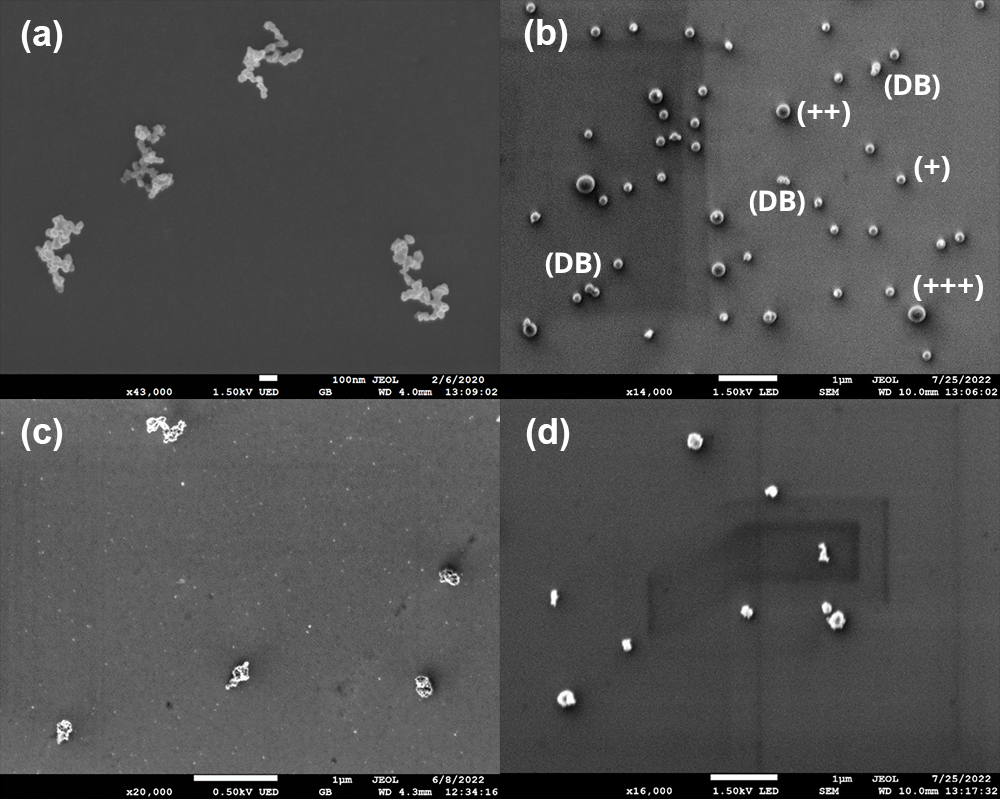
\includegraphics[width=\textwidth]{fig_sem.png}
\caption{SEM images of: (a) flame-generated soot, (b) nigrosin, (c) agglomerated CB, and (d) compact CB. In the image for nigrosin, (+), (++), and (+++) mark the singly, double, and triply charged particles with diameters of 147, 235, and 294 nm, respectively. Mobility diameters used to classify these particles: (a) 240 nm, (b) 150 nm, (c) 240 nm, and (d) 150 nm}
\label{fig:sem}
\end{figure}

The mass-mobility exponent can be determined from the dependence of the particle mass on the electrical mobility diameter (Equation \ref{eq:mass_prop}), where for non-fractal solid particles, mass is proportional to the cube of the linear dimension (diameter for spherical particles). This relationship can be written in relative form, where the electrical mobility diameter is normalized by a reference electrical mobility diameter, and mass is normalized by mass of particles of that reference electrical mobility diameter, allowing us to eliminate the proportionality constant (Equation \ref{eq:mass_mobility}).
\begin{equation}
    \label{eq:mass_prop}
    m\propto D^3
\end{equation}
\begin{equation}
    \label{eq:mass_mobility}
    \frac{m}{m_{\rm ref}}=\left(\frac{D}{D_{\rm ref}}\right)^\varepsilon
\end{equation}
Particle deviation from a spherical geometry causes the exponent in Equation \ref{eq:mass_mobility} to deviate from 3, while the overall power law dependence remains valid. Hence, we can define a general mass-mobility law, where $\varepsilon$ is mass-mobility exponent. It is important to note that $\varepsilon$ is a quantity similar to $D_f$, but is not equivalent.

To determine compactness, mass of particles of different electrical mobility diameters can be measured and $\varepsilon$ can be calculated by fitting the data to Equation \ref{eq:mass_mobility}. Such mass-mobility measurements were performed for the four aerosol types mentioned above and also for PSL, using 150 - 350 nm electrical mobility diameter particles (Figure \ref{fig:mass_mobility}). Perfectly spherical PSL particles produced mass mobility exponent of 3.00. Nigrosin particles, albeit spherical, produced  somewhat lower $\varepsilon$ approaching 2.95. Soot aggregates were highly fractal, with a mass-mobility exponent of 2.36. Carbon black particles fell between highly fractal soot and spherical nigrosin, with the mass-mobility exponent for compact CB closer to nigrosin (2.88) and that of agglomerated CB closer to soot (2.68).

\begin{figure}[htp]
    \centering
    \begin{tikzpicture}
    \begin{loglogaxis}[
    xlabel={$D,\ \rm nm$},
    ylabel={$m,\ \rm fg$},
    legend pos=north west,
    legend cell align={left},
    ymax=500,
    xtick={150,240,350},
    xticklabels={$150$,$240$,$350$}
    ]
        \addplot [only marks,color=tab_purple,mark=star] table {plots/mass_mobility_absolute/psl.txt};
        \addlegendentry{PSL, $\varepsilon=3.00$}
        % 1.0000    0.4980    0.0549
        \addplot [only marks,color=tab_orange,mark=square*] table {plots/mass_mobility_absolute/nigrosin.txt};
        \addlegendentry{Nigrosin, $\varepsilon=2.95$}
        \addplot [only marks,color=tab_grey,mark=triangle*] table {plots/mass_mobility_absolute/cb_cmp.txt};
        \addlegendentry{CB\textsubscript{cmp}, $\varepsilon=2.88$}
        \addplot [only marks,color=tab_red,mark=diamond*] table {plots/mass_mobility_absolute/cb_agg.txt};
        \addlegendentry{CB\textsubscript{agg}, $\varepsilon=2.68$}
        \addplot [only marks,color=tab_blue,mark=otimes*] table {plots/mass_mobility_absolute/soot.txt};
        \addlegendentry{Soot, $\varepsilon=2.36$}
        % PSL fit
        \addplot [domain=150:350,no markers,color=tab_purple] {5.386995e-07*x^3.004721};
        % Nigrosin fit
        \addplot [domain=150:350,no markers,color=tab_orange] {9.701697e-07*x^2.948992};
        % CB200_cmp fit
        \addplot [domain=150:350,no markers,color=tab_grey] {6.617110e-07*x^2.880935};
        % CB200_agg fit
        \addplot [domain=150:350,no markers,color=tab_red] {1.996164e-06*x^2.684836};
        % Soot fit
        \addplot [domain=150:350,no markers,color=tab_blue] {5.483814e-06*x^2.363773};
    \end{loglogaxis}
    \end{tikzpicture}
    \caption{Dependence of mass on the electrical mobility diameter for bare particles of different types. Listed mass mobility exponents ($\varepsilon$) are obtained from exponential fits.}
    \label{fig:mass_mobility}
\end{figure}

Mass-mobility measurements support the trend in convexities determined from SEM images and provide an alternative quantitative way to compare the morphology of different particle types. It is interesting to note that $\varepsilon$ for nigrosin is 2.95 and not exactly 3.00, as measured for PSL. Since imaging confirmed that nigrosin particles are spherical, the likely reason for this deviation is due to the contribution of multiply charged particles, as described in detail in the Supplemental Information (Section \ref{s:sec:multiple_charging_and_mass}).


\subsubsection{Particles processed by vapor condensation}

In coating experiments, mobility-classified particles of different types were exposed to supersaturated DOS vapor and then changes in the mobility diameter and mass were measured. The initial mobility diameters of the particles were chosen such that their initial volume equivalent diameters ($D_{ve}$) were approximately equal between the different types of aerosols used,
\begin{equation}
    \label{eq:diam_ve}
    D_{ve}=\sqrt[3]{\frac{6m}{\pi\rho}}
\end{equation}
where $m$ is particle mass and $\rho$ is material mass density. Electrical mobility and volume equivalent diameters, as well as particle masses and material mass densities, are provided in Table \ref{tab:densities}.

\begin{table}[ht]
\caption{Electrical mobility and volume-equivalent diameters of bare aerosol particles, along with particle mass and material mass density}
\label{tab:densities}
\begin{center}
\begin{tabular}{ l c c c c } 
 \hline
 & $D_m$, nm & $m$, fg & $\rho$, g/cm\textsuperscript{3} & $D_{ve}$, nm\\
 \hline
Soot & 240 & 2.367 & 1.77\textsuperscript{\textit{a}} & 137\\
Nigrosin & 150 & 2.488 & 1.41\textsuperscript{\textit{b}} & 150\\
CB (compact) & 150 & 1.283 & 1.77 & 111\\
CB (agglomerated) & 240 & 4.571 & 1.77 & 170\\
 \hline
\end{tabular}
\end{center}

\textsuperscript{\textit{a}} \citet{park2004measurement}\\
\textsuperscript{\textit{b}} Measured in this study (see mass-mobility measurements)
\end{table}



Fractal and compact particles responded differently to coating, as shown in Figure \ref{fig:gfd}a, where the dependence of electrical mobility diameter growth factor ($GF_d$) on mass growth factor ($GF_{ m}$) is plotted for coated aerosols. With the addition of DOS, $GF_d$ increased rapidly for nigrosin, but gradually for compact CB. For agglomerated CB, the value of $GF_d$ remained nearly unchanged (less than $1 \%$ change), increasing only slightly for $GF_m > 2$. In the case of soot, $GF_d$ decreased notably ($14\%$ decrease) for lower coating mass, but began to increase for $GF_m > 2.2$.

Compact CB particles grew less in mobility diameter than nigrosin particles for the same $GF_m$ because they are made of multiple smaller primary particles and contain significant void space, with an estimated void fraction of $60\%$, below the minimum void fraction of 36\% in fully compacted aggregates \citep{RN18}. Part of the DOS coating occupied the voids inside the compact CB particles instead of forming a layer around them, thus resulting in less size growth than for solid nigrosin spheres for the same relative increase in mass.

\begin{figure}[htp]
    \centering
    \resizebox{\columnwidth}{!}{\begin{tikzpicture}
    \begin{axis}[
    xlabel=$GF_m$,
    ylabel=$GF_d$,
    %legend pos=south east,
    xmin=1
    ]
        \addplot [color=tab_orange,mark=square*] table {plots/gfd/nigrosin_coated.txt};
        \addplot [color=tab_grey,mark=triangle*] table {plots/gfd/cb_cmp_coated.txt};
        \addplot [color=tab_red,mark=diamond*] table {plots/gfd/cb_agg_coated.txt};
        \addplot [color=tab_blue,mark=otimes*] table {plots/gfd/soot_coated.txt};
        \node[anchor=north east] at (rel axis cs:1,1) {\textbf{(a)}};
    \end{axis}
    \end{tikzpicture}
    \begin{tikzpicture}
    \begin{axis}[
    xlabel=$GF_m$,
    ylabel=$GF_d$,
    xmin=1,
    ymax=1.05,
    samples=2,
    legend cell align={left},
    legend style={at={(0.97,0.45)},anchor=east}
    ]
        \addplot [color=tab_orange,mark=square*][domain=0:3.5] {1};
        \addlegendentry{Nigrosin, $\rm 150\ nm$}
        \addplot [color=tab_grey,mark=triangle*] table {plots/gfd/cb_cmp_heated.txt};
        \addlegendentry{CB\textsubscript{cmp}, $\rm 150\ nm$}
        \addplot [color=tab_red,mark=diamond*] table {plots/gfd/cb_agg_heated.txt};
        \addlegendentry{CB\textsubscript{agg}, $\rm 240\ nm$}
        \addplot [color=tab_blue,mark=otimes*] table {plots/gfd/soot_heated.txt};
        \addlegendentry{Soot, $\rm 240\ nm$}
        \node[anchor=north east] at (rel axis cs:1,1) {\textbf{(b)}};
    \end{axis}
    \end{tikzpicture}}
    \caption{Electrical mobility diameter growth factor ($GF_d$) vs mass growth factor ($GF_{ m}$) upon processing of different types of particles: (a) DOS coated particles and (b) DOS-coated-denuded particles}
    \label{fig:gfd}
\end{figure}

Unlike compact particles, fractal soot and aggregated CB restructure upon condensation of DOS, with higher coating mass leading to greater compaction, as reflected by a decrease in $GF_d$. Since particle compaction is partially offset by the addition of the coating, the latter must be removed by thermal denuding to discriminate the contributions from restructuring and coating volume addition. As shown in Figure \ref{fig:gfd}b, the $GF_d$ of coated-denuded soot drops substantially, reaching nearly full compaction at $GF_m \approx 2$, as similarly reported in \citep{RN13}. By full compaction we refer to the minimum $GF_d$ that a soot aggregate can reach during restructuring. Only then the soot particle mobility diameter begins to increase during subsequent coating addition (Figure \ref{fig:gfd}a). In contrast to fractal soot, agglomerated CB particles undergo minimal restructuring, while for compact CB particles restructuring is barely noticeable. The negligible restructuring of compact CB is unsurprising because particles were generated from an aqueous suspension where aggregates underwent complete restructuring during manufacturing and upon droplet evaporation during nebulization \citep{RN51}. The somewhat more pronounced restructuring of agglomerated CB was due to partial folding of the branches (Figure \ref{fig:sem}c), each branch made of a compact CB particle (Figure \ref{fig:sem}d). These drastically different responses in volume equivalent coating thickness and morphology between particles of the four types produce different optical responses, as described in section \ref{sec:optical}.


\subsubsection{Growth by vapor condensation of multiply charged particles}

Multiply charged particles are larger and acquire coatings at a lower rate than the singly-charged smaller particles because in continuum regime the rate of vapor condensation is inversely proportional to particle radius \citep{RN2}, when the amount of coating is expressed in terms of coating thickness. This effect of slower coating thickness growth is less pronounced for fractal aggregates, at least while they remain lightly coated, because both singly charged smaller aggregates and multiply charged larger aggregates are composed of primary spherules of approximately the same diameter, which is smaller than the gas mean free path. Hence, individual primary spherules in both aggregates gain condensate under molecular condensation regime at the same rate. Experimentally, the slower rate of coating thickness growth of non-fractal multiply charged particles can be observed by adding a second diffusion charger after DMA1 during TDMA scans, allowing the discrimination between particles of different charges in the pseudo-monodisperse aerosol, as shown in Figure \ref{fig:recharged_coated} for fresh and coated nigrosin aerosol. Coating thicknesses calculated from mobility diameters of smaller and larger particles before and after coating application obtained from those scans (Table \ref{tab:recharged_coated}) indicate that the larger particles acquired a $24\%$ thinner coating layer.


\begin{figure}[htp]
    \centering
    \begin{tikzpicture}
    \begin{axis}[
    xlabel={$D/D_0\ \mathrm{nm}$},
    ylabel={$N,\ \rm cm^{-3}$},
    ymin=0,
    xmin=0.5,
    xmax=2,
    legend cell align={left}
    ]
        \addplot [only marks,tab_blue,mark=otimes*,mark options={scale=0.5}] table {plots/recharged_coated/nigrosin_fresh.txt} node [above,pos=0.33] {$1\rightarrow 2$} node [above,pos=0.5] {$q\rightarrow q$} node [above,pos=0.7] {$2\rightarrow 1$};
        \addplot [only marks,tab_orange,mark=square*,mark options={scale=0.5}] table {plots/recharged_coated/nigrosin_coated.txt};
        % f(x) mult/stdev/sqrt(2*pi)*exp(-1/2*((x-shift)./stdev).^2)
        \addplot [domain=0.5:2,no markers,color=tab_blue,samples=100] {0.3972/0.0425/sqrt(2*pi)*exp(-1/2*((x-0.6746)/0.0425)^2)+2.4380/0.0634/sqrt(2*pi)*exp(-1/2*((x-1.0230)/0.0634)^2)+0.7397/0.1165/sqrt(2*pi)*exp(-1/2*((x-1.5875)/0.1165)^2)};
        \addplot [domain=0.5:2,no markers,color=tab_orange,samples=100] {0.4535/0.0504/sqrt(2*pi)*exp(-1/2*((x-0.7762)/0.0504)^2)+2.8188/0.0782/sqrt(2*pi)*exp(-1/2*((x-1.1878)/0.0782)^2)+0.9328/0.1457/sqrt(2*pi)*exp(-1/2*((x-1.7128)/0.1457)^2)};
        \addlegendentry{Fresh};
        \addlegendentry{Coated};
    \end{axis}
    \end{tikzpicture}
    \caption{Recharged TDMA scans of fresh and coated 150 nm nigrosin. X-axis, the electrical mobility diameter, is normalized by $D_0=150\ \rm nm$. $q\rightarrow q$ indicates particles that were singly charged prior to recharging and remained singly charged after, but this mode still contains a significant number of doubly charged particles \citep{RN7}, $2\rightarrow 1$ indicates particles that were doubly charged prior to recharging and became singly charged after, $1\rightarrow 2$ indicates particles that were singly charged prior to recharging and became doubly charged after. While there are also triply charged particles in the size-classified aerosol, they are not visible in this TDMA scan due to limitations on the scan range with the sample flow rate used during optical measurements. Broader scans of bare particles that do show triply charged particles are available in Figure \ref{s:fig:recharged_all}.}
    \label{fig:recharged_coated}
\end{figure}

\begin{table}[htp]
    \centering
    \caption{Coating thickness of singly and doubly charged nigrosin particles of 150 nm initial mobility diameter (data from Figure \ref{fig:recharged_coated})}
    \begin{tabular}{c c c c}
        \hline
        & $1\rightarrow 2$ & $1\rightarrow 1$ & $2\rightarrow 1$ \\
        \hline
        $GF_{d,\rm bare}$ & 0.673 & 1.020 & 1.587\\
        $GF_{d,\rm coated}$ & 0.773 & 1.187 & 1.713\\
        $D_{\mathrm{bare}}$, nm & 154 & 153 & 238 \\
        $D_{\mathrm{coated}}$, nm & 178 & 178 & 257 \\
        $\Delta r_{ve}$, nm & 12.0 & 12.5 & 9.5 \\
        \hline
    \end{tabular}
    \label{tab:recharged_coated}
\end{table}

\subsection{Optical measurements}

\label{sec:optical}

\subsubsection{The effect of multiple charging on measured optical cross sections of bare particles}

We begin our discussion with analysis of absolute optical cross sections, which often are subject to significant uncertainty. A major source of this uncertainty stems from size classification of particles based on their electrical mobility, which may introduce a significant fraction of particles carrying multiple charges in a nominally monodisperse aerosol. As described in the previous section, such particles are larger than the particles of interest and hence absorb and scatter light stronger, resulting in an overestimation of these optical properties. The contribution from these multiply charged particles must be accounted for when deriving absolute absorption and scattering cross sections, optical enhancements, and single-scattering albedo (SSA), as described below.

Most commonly, the size-classified aerosol is passed through a second diffusion charger, which re-charges the particles and allows to reveal the nearly-true distribution of multiply-charged particles among the size-selected particles on a TDMA scan. Alternatively, one can use electron microscopy images of particle samples to estimate fractions of larger multiply charged particles, at least for non-fractal particles of regular shapes. When the aerosol number concentration is low, the contribution from some particle modes, such as from triply charged particles is difficult to quantify accurately, but their contribution to measured scattering and absorption cross sections can still be significant. Below we illustrate the application of both approaches, recharging-TDMA and SEM imaging, towards elucidating the fraction of multiply charged particles in a nominally monodisperse sample of spherical nigrosin particles, and evaluating the contribution of such particles to absorption and scattering cross sections.

Based on the recharged TDMA scan of the 150 nm mobility diameter nigrosin  shown in Figure \ref{s:fig:recharged_all}b and using equations \ref{s:eq:gaussian-mode} - \ref{s:eq:gaussian-fraction}, number fractions ($f_i$) of singly, doubly, and triply charged particles were found to be 76\%, 19\%, and 5\%, respectively. The sizes of these particles were 150, 236, and 315 nm, corresponding to the peaks at 1.02, 1.59, and 2.11 in the TDMA scan (Figure \ref{s:fig:recharged_all}b). Counting particles of three different sizes in the SEM image (Figure \ref{fig:sem}b) provided similar albeit not identical fractions, $84\%$, $11\%$, and $4\%$. The difference between the two methods is a result of several effects, including insufficient statistics due to the small number of examined particles in the SEM image and the non-negligible ``contamination'' of the $1\rightarrow 1$ particle mode in Figure \ref{s:fig:recharged_all}b by doubly charged particles \citep{RN7}. Unlike this ``contamination'', the statistics can be improved by increasing the number of interrogated particles, and hence in the following example we use the fractions obtained from the SEM image to calculate the contributions to absorption and scattering cross sections from each individual particle mode, along with the total cross sections comprising the sum of all three modes,
\begin{equation}
    C_\mathrm{abs/sca,tot}=\sum_{i}{f_iC_{\mathrm{abs/sca},i}}
    \label{eq:total_corss_section}
\end{equation}
where $f_i$ is the number fraction of the respective mode, $C_{\mathrm{abs/sca},i}$ is the absorption or scattering cross section of the respective mode, and $C_{\rm abs/sca,tot}$ is the overall scattering or absorption cross section of the aerosol. The relative contribution of mode $i$ to total cross section is

\begin{equation}
    f_{\mathrm{abs/sca}}=\frac{C_{\mathrm{abs/sca},i}\times f_i}{C_\mathrm{abs/sca,tot}}
    \label{eq:contribution}
\end{equation}

As shown in Table \ref{tab:absorption_mie}, triply charged nigrosin particles, being only $4\%$ by number, contributed to $22\%$ of the total absorption cross section and $34\%$ of the total scattering cross section. The total estimated absorption cross section including all three modes is $1.78\times 10^{-14}\ \mathrm{m}^2$, while the absorption cross section consisting only of 150 nm particles is $1.04\times 10^{-14}\ \mathrm{m}^2$. Thus, presence of doubly and triply charged particles in a mobility-classified aerosol leads to overestimation of the absorption cross section by $71\%$. The bias due to larger particle modes is even more significant for scattering, where the total estimated scattering cross section is $1.36\times 10^{-14}\ \mathrm{m}^2$, while the scattering cross section of the 150 nm particle mode is $5.06\times 10^{-15}\ \mathrm{m}^2$, indicating a $169\%$ overestimation. For comparison, experimentally measured absorption and scattering cross sections for 150 nm nigrosin measured without recharging were $2.00\times 10^{-14}\ \mathrm{m}^2$ and $1.87\times 10^{-14}\ \mathrm{m}^2$ respectively. Thus, factoring the optical contributions of multiply charged particles into calculated optical properties reduced the bias, but still failed to provide full agreement for a number of reasons, e.g., the singly-charged particle mode in Figure \ref{s:fig:recharged_all}b still containing a fraction of doubly charged particles \citep{RN7}, the presence of particles with higher order charges that could not be detected due to their large size and small number density, etc.

\begin{table}[htp]
    \centering
    \caption{Absorption and scattering characteristics of nigrosin particles calculated with Mie. Quantitative statistics are based on particle counts from the SEM image shown in Figure \ref{fig:sem}b.}
    \begin{tabular}{l c c c}
        \hline
        & 150 nm & 236 nm & 315 nm \\
        \hline
        Number fraction ($f_i$) & 0.84 & 0.11 & 0.04 \\
        Particle mass, fg & 2.49 & 9.70 & 23.08 \\
        \multicolumn{4}{c}{\textit{Absorption}} \\
        \hline
        $C_{\mathrm{abs}},\ \mathrm{m}^2\times10^{14}$ & 1.04 & 4.70 & 9.64 \\
        $C_{\mathrm{abs}}\times f_i,\ \mathrm{m}^2\times10^{14}$ & 0.876 & 0.517 & 0.386 \\
        Contribution, $C_{\mathrm{abs}}\times f\over C_{\mathrm{abs,total}}$ & 0.493 & 0.291 & 0.217 \\
        MAC, $\mathrm{m}^2/\mathrm{g}$ & 4.19 & 4.48 & 4.18 \\
        $C_{\rm abs,tot},\ \rm m^2\times10^{14}$ & \multicolumn{3}{c}{1.78 (total of three modes)} \\
        \multicolumn{4}{c}{\textit{Scattering}} \\
        \hline
        $C_\mathrm{sca},\ \mathrm{m}^2\times 10^{14}$ & 0.506 & 4.32 & 11.6 \\
        $C_\mathrm{sca}\times f_i,\ \mathrm{m}^2\times 10^{14}$ & 0.425 & 0.475 & 0.464 \\
        Contribution, $C_\mathrm{sca}\times f_i\over C_\mathrm{sca,tot}$ & 0.312 & 0.348 & 0.340 \\
        $C_{\rm sca,tot},\ \rm m^2\times10^{14}$ & \multicolumn{3}{c}{1.36 (total of three modes)} \\
        \hline
    \end{tabular}
    \label{tab:absorption_mie}
\end{table}

One can physically reduce the fraction of multiply charged particles in a mobility-classified aerosol by selecting particles with diameters that are on the falling edge (or towards the tail end) of the incoming aerosol size distribution (Figure \ref{s:fig:smps}). As shown in Figure \ref{s:fig:recharged_all}, whereas 150 nm electrical mobility classified aerosols of different types contain large fractions of doubly charged particles, the fraction of those particles is significantly lower in the 240 nm aerosols. Hence, a simple way to minimize the contribution of multiply charged particles during experimental measurements is by carefully selecting the target particle size during mobility classification. In the following section, we explore how the presence of multiply charged particles affects the relative optical enhancements when bare particles become coated.

\subsubsection{Optical response of coated particles}

Figure \ref{fig:opt_data} shows experimentally measured enhancements in light absorption and scattering for the different particle types subjected to processing via coating by DOS (a, c, e) or coating combined with thermal denuding (b, d, f), along with the corresponding changes in SSA. The enhancements were obtained by normalizing experimentally measured optical cross sections of processed aerosols by optical cross sections of bare aerosols. The SSA was calculated as a ratio of scattering and extinction cross sections for the same aerosol, either fresh or processed. Presenting data in a normalized form facilitates comparison of different particle types, which have significantly different absolute values of absorption and scattering cross sections (see Figure \ref{s:fig:mie_abs}). Also, such representation is common for optical data reporting in laboratory, field, and computational studies \citep{RN7,RN52,RN22}.

\begin{figure}[htp]
    \centering
    \resizebox{\columnwidth}{!}{\begin{tikzpicture}
    \begin{axis}[
    xlabel={$\Delta r_\mathrm{ve},\ \mathrm{nm}$},
    ylabel=$E_\mathrm{abs}$,
    legend pos=south east,
    xmin=0,
    ymin=1,
    legend cell align={left}
    ]
        \addplot [color=tab_orange,mark=square*,error bars/.cd, y dir=both, y explicit] table [col sep=tab,y=E_abs,y error=E_abs_err] {plots/enhancements_experiment/nigrosin.txt};
        \addlegendentry{Nigrosin}
        \addplot [color=tab_grey,mark=triangle*,error bars/.cd, y dir=both, y explicit] table [col sep=tab,y=E_abs,y error=E_abs_err] {plots/enhancements_experiment/cb_cmp_coated.txt};
        \addlegendentry{CB200\textsubscript{cmp}}
        \addplot [color=tab_red,mark=diamond*,error bars/.cd, y dir=both, y explicit] table [col sep=tab,y=E_abs,y error=E_abs_err] {plots/enhancements_experiment/cb_agg_coated.txt};
        \addlegendentry{CB200\textsubscript{agg}}
        \addplot [color=tab_blue,mark=otimes*,error bars/.cd, y dir=both, y explicit] table [col sep=tab,y=E_abs,y error=E_abs_err] {plots/enhancements_experiment/soot_coated.txt};
        \addlegendentry{Soot}
        \node[anchor=north east] at (rel axis cs:1,1) {\textbf{(a)}};
    \end{axis}
    \end{tikzpicture}
    \begin{tikzpicture}
    \begin{axis}[
    xlabel={$\Delta r_\mathrm{ve},\ \mathrm{nm}$},
    ylabel=$E_\mathrm{abs}$,
    xmin=0
    ]
        \addplot [color=tab_grey,mark=triangle*,error bars/.cd, y dir=both, y explicit] table [col sep=tab,y=E_abs,y error=E_abs_err] {plots/enhancements_experiment/cb_cmp_heated.txt};
        \addplot [color=tab_red,mark=diamond*,error bars/.cd, y dir=both, y explicit] table [col sep=tab,y=E_abs,y error=E_abs_err] {plots/enhancements_experiment/cb_agg_heated.txt};
        \addplot [color=tab_blue,mark=otimes*,error bars/.cd, y dir=both, y explicit] table [col sep=tab,y=E_abs,y error=E_abs_err] {plots/enhancements_experiment/soot_heated.txt};
        \node[anchor=north east] at (rel axis cs:1,1) {\textbf{(b)}};
    \end{axis}
    \end{tikzpicture}}
    \resizebox{\columnwidth}{!}{\begin{tikzpicture}
    \begin{axis}[
    xlabel={$\Delta r_\mathrm{ve},\ \mathrm{nm}$},
    ylabel=$E_\mathrm{sca}$,
    xmin=0,
    ymin=1
    ]
        \addplot [color=tab_orange,mark=square*,error bars/.cd, y dir=both, y explicit] table [col sep=tab,y=E_sca,y error=E_sca_err] {plots/enhancements_experiment/nigrosin.txt};
        \addplot [color=tab_grey,mark=triangle*,error bars/.cd, y dir=both, y explicit] table [col sep=tab,y=E_sca,y error=E_sca_err] {plots/enhancements_experiment/cb_cmp_coated.txt};
        \addplot [color=tab_red,mark=diamond*,error bars/.cd, y dir=both, y explicit] table [col sep=tab,y=E_sca,y error=E_sca_err] {plots/enhancements_experiment/cb_agg_coated.txt};
        \addplot [color=tab_blue,mark=otimes*,error bars/.cd, y dir=both, y explicit] table [col sep=tab,y=E_sca,y error=E_sca_err] {plots/enhancements_experiment/soot_coated.txt};
        \node[anchor=north east] at (rel axis cs:1,1) {\textbf{(c)}};
    \end{axis}
    \end{tikzpicture}
    \begin{tikzpicture}
    \begin{axis}[
    xlabel={$\Delta r_\mathrm{ve},\ \mathrm{nm}$},
    ylabel=$E_\mathrm{sca}$,
    xmin=0
    ]
        \addplot [color=tab_grey,mark=triangle*,error bars/.cd, y dir=both, y explicit] table [col sep=tab,y=E_sca,y error=E_sca_err] {plots/enhancements_experiment/cb_cmp_heated.txt};
        \addplot [color=tab_red,mark=diamond*,error bars/.cd, y dir=both, y explicit] table [col sep=tab,y=E_sca,y error=E_sca_err] {plots/enhancements_experiment/cb_agg_heated.txt};
        \addplot [color=tab_blue,mark=otimes*,error bars/.cd, y dir=both, y explicit] table [col sep=tab,y=E_sca,y error=E_sca_err] {plots/enhancements_experiment/soot_heated.txt};
        \node[anchor=north east] at (rel axis cs:1,1) {\textbf{(d)}};
    \end{axis}
    \end{tikzpicture}}
    \resizebox{\columnwidth}{!}{\begin{tikzpicture}
    \begin{axis}[
    xlabel={$\Delta r_\mathrm{ve},\ \mathrm{nm}$},
    ylabel=$\rm SSA$,
    xmin=0,
    ymin=0.2,
    ymax=0.7
    ]
        \addplot [color=tab_orange,mark=square*,error bars/.cd, y dir=both, y explicit] table [col sep=tab,y=SSA,y error=SSA_err] {plots/absolute_experimental/nigrosin.txt};
        \addplot [color=tab_grey,mark=triangle*,error bars/.cd, y dir=both, y explicit] table [col sep=tab,y=SSA,y error=SSA_err] {plots/absolute_experimental/cb_cmp_coated.txt};
        \addplot [color=tab_red,mark=diamond*,mark=otimes*,error bars/.cd, y dir=both, y explicit] table [col sep=tab,y=SSA,y error=SSA_err] {plots/absolute_experimental/cb_agg_coated.txt};
        \addplot [color=tab_blue,mark=otimes*,error bars/.cd, y dir=both, y explicit] table [col sep=tab,y=SSA,y error=SSA_err] {plots/absolute_experimental/soot_coated.txt};
        \node[anchor=north east] at (rel axis cs:1,1) {\textbf{(e)}};
    \end{axis}
    \end{tikzpicture}
    \begin{tikzpicture}
    \begin{axis}[
    xlabel={$\Delta r_\mathrm{ve},\ \mathrm{nm}$},
    ylabel=$\rm SSA$,
    xmin=0,
    ymin=0.2,
    ymax=0.7
    ]
        \addplot [color=tab_grey,mark=triangle*,error bars/.cd, y dir=both, y explicit] table [col sep=tab,y=SSA,y error=SSA_err] {plots/absolute_experimental/cb_cmp_heated.txt};
        \addplot [color=tab_red,mark=diamond*,mark=otimes*,error bars/.cd, y dir=both, y explicit] table [col sep=tab,y=SSA,y error=SSA_err] {plots/absolute_experimental/cb_agg_heated.txt};
        \addplot [color=tab_blue,mark=otimes*,error bars/.cd, y dir=both, y explicit] table [col sep=tab,y=SSA,y error=SSA_err] {plots/absolute_experimental/soot_heated.txt};
        \node[anchor=north east] at (rel axis cs:1,1) {\textbf{(f)}};
    \end{axis}
    \end{tikzpicture}}
    \caption{Experimentally measured enhancement in light absorption (a, b), scattering (c, d), and SSA (e, f) for coated (a, c, e) and coated-denuded (b, d, f) aerosols of different types. Relative error for optical cross sections ranges from 5\% (for bare particles with weak scattering signal) to 1\% (for thickly coated particles with strong scattering and extinction)}
    \label{fig:opt_data}
\end{figure}



The addition of coating enhances light absorption for all particle types (Figure \ref{fig:opt_data}a), with the largest enhancement ($E_{\rm abs}=1.30$) observed for spherical nigrosin particles and the lowest ($E_{\rm abs}=1.15$) for fractal soot particles for a 30 nm thick coating (volume equivalent coating thickness, as defined by Equation \ref{eq:drve})). For soot, the magnitude of enhancement is in agreement with previous experimental measurements \citep{RN41,RN7}. The enhancement in light scattering is more substantial than for absorption (Figure \ref{fig:opt_data}c), with the largest values observed for fractal soot ($E_{sca} = 3.5$ at 30 nm coating thickness), followed by the other particle types ($E_{\rm sca} \approx 2$). During coating, absorption and scattering can be altered by changes in both the particle mixing state (addition of a coating layer) and morphology (restructuring), with the exception of nigrosin, where only the mixing state is altered. By removing the coating layer via thermal denuding, it is possible to isolate changes induced by the restructured particle morphology from the changes due to coating addition.

Thermal denuding of coated particles reduces the enhancement in absorption to 1.00±0.05 for all particle types (Figure \ref{fig:opt_data}). Thus, absorption is largely independent of the soot particle morphology but can be significantly increased by the lensing effect, where the transparent coating layer intensifies light absorption by the particle core.
%indicating that absorption is not affected significantly by restructuring of fractal soot aggregates \citep{RN53} and the major cause of enhancement is the lensing effect, where the transparent shell of coating material makes light absorption by the particle core stronger \citep{RN34}.
Scattering enhancement also decreases after denuding, approaching unity for all particle types except for soot ($E_{sca} = 1.45$ at 30 nm coating thickness), as shown in Figure \ref{fig:opt_data}d. The significant residual scattering enhancement in soot is the result of restructuring experienced by fractal particles. As shown previously \citep{RN40}, the primary particles in fractal aggregates scatter light poorly due to their small size relative to the light wavelength, but after restructuring the interactions between the primary particles increase, leading to a significant increase in scattering \citep{RN7}. The more fractal the particle is initially, the higher the increase in scattering will be after processing. The joint effect of restructuring and lensing is responsible for fractal soot having the largest scattering enhancement during coating.

For bare particles, SSA is the lowest for fractal soot and the highest for nigrosin (Figure \ref{fig:opt_data}e). With the addition of the coating shell, SSA increases with approximately the same slope for all particle types, although fractal soot shows a faster rate of increase in the 15-30 nm region, where it undergoes significant restructuring. This region can be clearly seen in experiments with coated-denuded soot (Figure \ref{fig:opt_data}f). For other particle types, SSA of bare and coated-denuded particles remain unchanged within experimental uncertainty.


\subsubsection{Comparison of experiments with simple optics models}

Figures \ref{fig:mie_abs} and \ref{fig:mie_sca} compare experimentally measured absorption and scattering enhancements for all particle types against calculations by the commonly used core-shell Mie optical model, which predicts optical properties exactly for spherical particles and often produces a reasonable agreement for compact aggregates. In the case of soot and CB, we also included the calculation by the RDG-Mie approach.

%but which underestimates absorption because it neglects the spherule-spherule coupling.

When comparing experiments against Mie calculations, the agreement in absorption enhancement is better for nigrosin and aggregated CB (Figure \ref{fig:mie_abs}b and \ref{fig:mie_abs}d) than for soot and compact CB (Figure \ref{fig:mie_abs}a and \ref{fig:mie_abs}c), especially at coating thicknesses below 25 nm. The RDG-Mie values agree with measured absorption enhancement for soot with coating thicknesses below 30 nm, but become lower than experimental values for thicker coatings. Such a trend can be readily explained by the fact that, for absorption, the RDG approach assumes no optical interaction between primary particles. This assumption is approximately valid for fractal aggregates, but not for compact aggregates. For this reason, RDG-Mie performed poorly in predicting absorption enhancement for both types of CB particles. For scattering enhancement predicted by Mie, there was a reasonable agreement with experimental measurements for soot and agglomerated CB, (Figures \ref{fig:mie_sca}a,d), but for nigrosin and compact CB the deviation was high and the curves diverged progressively with increasing coating thickness. SSA was significantly underestimated by Mie calculations for all aerosol types (Figure \ref{fig:ssa}), with the lowest deviation in the case of fractal soot.

Many factors can contribute to differences in experimental optical measurements for soot and its surrogates and also to disagreement between the experimental optical measurements and optical model predictions. These factors include differences in particle morphology between soot and its surrogates, the presence of multiply charged larger particles in nominally size-classified aerosol, and an implicit assumption that singly and larger multiply-charged particles acquire coatings at the same rate \citep{RN75}. In the following, we assess and discuss contributions from some of these factors.

\begin{figure}[htp]
    \centering
    \resizebox{\columnwidth}{!}{\begin{tikzpicture}
    \begin{axis}[
    xlabel={$\Delta r_\mathrm{ve},\ \mathrm{nm}$},
    ylabel=$E_\mathrm{abs}$,
    legend pos=north west,
    xmin=0,
    ymin=1,
    legend cell align={left}
    ]
        \addplot [only marks,color=tab_blue,mark=otimes*,error bars/.cd, y dir=both, y explicit] table [col sep=tab,y=E_abs,y error=E_abs_err] {plots/enhancements_experiment/soot_coated.txt};
        \addlegendentry{Experimental}
        \addplot [no markers,color=tab_blue] table [col sep=tab,y=E_abs_mie] {plots/enhancements_mie/soot.txt};
        \addlegendentry{Mie (+)}
        \addplot [ultra thick,dashed,no markers,color=tab_blue] table [col sep=tab,y=E_abs_corr] {plots/enhancements_mie/soot.txt};
        \addlegendentry{Mie (+,++)}
        \addplot [ultra thick,dotted,no markers,color=tab_blue] table [col sep=tab,y=E_abs_rdg] {plots/enhancements_mie/soot.txt};
        \addlegendentry{RDG/Mie}
        \node[anchor=north east] at (rel axis cs:1,1) {\textbf{(a)}};
        \node[anchor=south east] at (rel axis cs:1,0) {\textbf{Soot}};
    \end{axis}
    \end{tikzpicture}
    \begin{tikzpicture}
    \begin{axis}[
    xlabel={$\Delta r_\mathrm{ve},\ \mathrm{nm}$},
    ylabel=$E_\mathrm{abs}$,
    legend pos=north west,
    xmin=0,
    ymin=1,
    legend cell align={left}
    ]
        \addplot [only marks,color=tab_orange,mark=square*,error bars/.cd, y dir=both, y explicit] table [col sep=tab,y=E_abs,y error=E_abs_err] {plots/enhancements_experiment/nigrosin.txt};
        \addplot [no markers,color=tab_orange] table [col sep=tab,y=E_abs_mie] {plots/enhancements_mie/nigrosin.txt};
        \addplot [ultra thick,dashed,no markers,color=tab_orange] table [col sep=tab,y=E_abs_corr] {plots/enhancements_mie/nigrosin.txt};
        \node[anchor=north east] at (rel axis cs:1,1) {\textbf{(b)}};
        \node[anchor=south east] at (rel axis cs:1,0) {\textbf{Nigrosin}};
    \end{axis}
    \end{tikzpicture}}
    \resizebox{\columnwidth}{!}{\begin{tikzpicture}
    \begin{axis}[
    xlabel={$\Delta r_\mathrm{ve},\ \mathrm{nm}$},
    ylabel=$E_\mathrm{abs}$,
    legend pos=north west,
    xmin=0,
    ymin=1,
    legend cell align={left}
    ]
        \addplot [only marks,color=tab_grey,mark=triangle*,error bars/.cd, y dir=both, y explicit] table [col sep=tab,y=E_abs,y error=E_abs_err] {plots/enhancements_experiment/cb_cmp_coated.txt};
        \addplot [no markers,color=tab_grey] table [col sep=tab,y=E_abs_mie] {plots/enhancements_mie/cb_cmp.txt};
        \addplot [ultra thick,dashed,no markers,color=tab_grey] table [col sep=tab,y=E_abs_corr] {plots/enhancements_mie/cb_cmp.txt};
        \addplot [ultra thick,dotted,no markers,color=tab_grey] table [col sep=tab,y=E_abs_rdg] {plots/enhancements_mie/cb_cmp.txt};
        \node[anchor=north east] at (rel axis cs:1,1) {\textbf{(c)}};
        \node[anchor=south east] at (rel axis cs:1,0) {\textbf{CB\textsubscript{cmp}}};
    \end{axis}
    \end{tikzpicture}
    \begin{tikzpicture}
    \begin{axis}[
    xlabel={$\Delta r_\mathrm{ve},\ \mathrm{nm}$},
    ylabel=$E_\mathrm{abs}$,
    legend pos=north west,
    xmin=0,
    ymin=1,
    legend cell align={left}
    ]
        \addplot [only marks,color=tab_red,mark=diamond*,error bars/.cd, y dir=both, y explicit] table [col sep=tab,y=E_abs,y error=E_abs_err] {plots/enhancements_experiment/cb_agg_coated.txt};
        \addplot [no markers,color=tab_red] table [col sep=tab,y=E_abs_mie] {plots/enhancements_mie/cb_agg.txt};
        \addplot [ultra thick,dashed,no markers,color=tab_red] table [col sep=tab,y=E_abs_corr] {plots/enhancements_mie/cb_agg.txt};
        \addplot [ultra thick,dotted,no markers,color=tab_red] table [col sep=tab,y=E_abs_rdg] {plots/enhancements_mie/cb_agg.txt};
        \node[anchor=north east] at (rel axis cs:1,1) {\textbf{(d)}};
        \node[anchor=south east] at (rel axis cs:1,0) {\textbf{CB\textsubscript{agg}}};
    \end{axis}
    \end{tikzpicture}}
    \caption{Measured and calculated absorption enhancements for compact soot (a), nigrosin (b), compact CB (c), and agglomerated CB (d). Measured data are presented by markers, calculated with Mie theory by solid line, and calculated with Mie by accounting for doubly charged particles by dashed line. For cases (a) and (d), the dashed and solid line overlap due to a negligible fraction of double charged particles. Volume equivalent and mobility diameters for all aerosol types are available in Table \ref{tab:densities}.}
    \label{fig:mie_abs}
\end{figure}

\begin{figure}[htp]
    \centering
    \resizebox{\columnwidth}{!}{\begin{tikzpicture}
    \begin{axis}[
    xlabel={$\Delta r_\mathrm{ve},\ \mathrm{nm}$},
    ylabel=$E_\mathrm{sca}$,
    legend pos=north west,
    xmin=0,
    ymin=1,
    legend cell align={left}
    ]
        \addplot [only marks,color=tab_blue,mark=otimes*,error bars/.cd, y dir=both, y explicit] table [col sep=tab,y=E_sca,y error=E_sca_err] {plots/enhancements_experiment/soot_coated.txt};
        \addlegendentry{Experimental}
        \addplot [no markers,color=tab_blue] table [col sep=tab,y=E_sca_mie] {plots/enhancements_mie/soot.txt};
        \addlegendentry{Mie (+)}
        \addplot [ultra thick,dashed,no markers,color=tab_blue] table [col sep=tab,y=E_sca_corr] {plots/enhancements_mie/soot.txt};
        \addlegendentry{Mie (+,++)}
        \node[anchor=north east] at (rel axis cs:1,1) {\textbf{(a)}};
        \node[anchor=south east] at (rel axis cs:1,0) {\textbf{Soot}};
    \end{axis}
    \end{tikzpicture}
    \begin{tikzpicture}
    \begin{axis}[
    xlabel={$\Delta r_\mathrm{ve},\ \mathrm{nm}$},
    ylabel=$E_\mathrm{sca}$,
    legend pos=north west,
    xmin=0,
    ymin=1,
    legend cell align={left}
    ]
        \addplot [only marks,color=tab_orange,mark=square*,error bars/.cd, y dir=both, y explicit] table [col sep=tab,y=E_sca,y error=E_sca_err] {plots/enhancements_experiment/nigrosin.txt};
        \addplot [no markers,color=tab_orange] table [col sep=tab,y=E_sca_mie] {plots/enhancements_mie/nigrosin.txt};
        \addplot [ultra thick,dashed,no markers,color=tab_orange] table [col sep=tab,y=E_sca_corr] {plots/enhancements_mie/nigrosin.txt};
        \node[anchor=north east] at (rel axis cs:1,1) {\textbf{(b)}};
        \node[anchor=south east] at (rel axis cs:1,0) {\textbf{Nigrosin}};
    \end{axis}
    \end{tikzpicture}}
    \resizebox{\columnwidth}{!}{\begin{tikzpicture}
    \begin{axis}[
    xlabel={$\Delta r_\mathrm{ve},\ \mathrm{nm}$},
    ylabel=$E_\mathrm{sca}$,
    legend pos=north west,
    xmin=0,
    ymin=1,
    legend cell align={left}
    ]
        \addplot [only marks,color=tab_grey,mark=triangle*,error bars/.cd, y dir=both, y explicit] table [col sep=tab,y=E_sca,y error=E_sca_err] {plots/enhancements_experiment/cb_cmp_coated.txt};
        \addplot [no markers,color=tab_grey] table [col sep=tab,y=E_sca_mie] {plots/enhancements_mie/cb_cmp.txt};
        \addplot [ultra thick,dashed,no markers,color=tab_grey] table [col sep=tab,y=E_sca_corr] {plots/enhancements_mie/cb_cmp.txt};
        \node[anchor=north east] at (rel axis cs:1,1) {\textbf{(c)}};
        \node[anchor=south east] at (rel axis cs:1,0) {\textbf{CB\textsubscript{cmp}}};
    \end{axis}
    \end{tikzpicture}
    \begin{tikzpicture}
    \begin{axis}[
    xlabel={$\Delta r_\mathrm{ve},\ \mathrm{nm}$},
    ylabel=$E_\mathrm{sca}$,
    legend pos=north west,
    xmin=0,
    ymin=1,
    legend cell align={left}
    ]
        \addplot [only marks,color=tab_red,mark=diamond*,error bars/.cd, y dir=both, y explicit] table [col sep=tab,y=E_sca,y error=E_sca_err] {plots/enhancements_experiment/cb_agg_coated.txt};
        \addplot [no markers,color=tab_red] table [col sep=tab,y=E_sca_mie] {plots/enhancements_mie/cb_agg.txt};
        \addplot [ultra thick,dashed,no markers,color=tab_red] table [col sep=tab,y=E_sca_corr] {plots/enhancements_mie/cb_agg.txt};
        \node[anchor=north east] at (rel axis cs:1,1) {\textbf{(d)}};
        \node[anchor=south east] at (rel axis cs:1,0) {\textbf{CB\textsubscript{agg}}};
    \end{axis}
    \end{tikzpicture}}
    \caption{Measured and calculated scattering  enhancements for compact soot (a), nigrosin (b), compact CB (c), and agglomerated CB (d). Measured data are shown by markers, calculated with Mie theory by solid line, and calculated with Mie by accounting for doubly charged particles by dashed line. For cases (a) and (d), the dashed and solid line overlap due to a negligible fraction of double charged particles. Volume equivalent and mobility diameters for all aerosol types are available in Table \ref{tab:densities}}
    \label{fig:mie_sca}
\end{figure}

\begin{figure}[htp]
    \centering
    \resizebox{\columnwidth}{!}{\begin{tikzpicture}
    \begin{axis}[
    xlabel={$\Delta r_\mathrm{ve},\ \mathrm{nm}$},
    ylabel=$\rm SSA$,
    legend pos=north west,
    xmin=0,
    legend cell align={left}
    ]
        \addplot [only marks,color=tab_blue,mark=otimes*,error bars/.cd, y dir=both, y explicit] table [col sep=tab,y=SSA,y error=SSA_err] {plots/absolute_experimental/soot_coated.txt};
        \addlegendentry{Experimental}
        \addplot [no markers,color=tab_blue] table [col sep=tab,y=SSA_mie] {plots/absolute_mie/soot.txt};
        \addlegendentry{Mie (+)}
        \addplot [ultra thick,dashed,no markers,color=tab_blue] table [col sep=tab,y=SSA_corr] {plots/absolute_mie/soot.txt};
        \addlegendentry{Mie (+,++)}
        \node[anchor=north east] at (rel axis cs:1,1) {\textbf{(a)}};
        \node[anchor=south east] at (rel axis cs:1,0) {\textbf{Soot}};
    \end{axis}
    \end{tikzpicture}
    \begin{tikzpicture}
    \begin{axis}[
    xlabel={$\Delta r_\mathrm{ve},\ \mathrm{nm}$},
    ylabel=$\rm SSA$,
    legend pos=north west,
    xmin=0,
    legend cell align={left}
    ]
        \addplot [only marks,color=tab_orange,mark=square*,error bars/.cd, y dir=both, y explicit] table [col sep=tab,y=SSA,y error=SSA_err] {plots/absolute_experimental/nigrosin.txt};
        \addplot [no markers,color=tab_orange] table [col sep=tab,y=SSA_mie] {plots/absolute_mie/nigrosin.txt};
        \addplot [ultra thick,dashed,no markers,color=tab_orange] table [col sep=tab,y=SSA_corr] {plots/absolute_mie/nigrosin.txt};
        \node[anchor=north east] at (rel axis cs:1,1) {\textbf{(b)}};
        \node[anchor=south east] at (rel axis cs:1,0) {\textbf{Nigrosin}};
    \end{axis}
    \end{tikzpicture}}
    \resizebox{\columnwidth}{!}{\begin{tikzpicture}
    \begin{axis}[
    xlabel={$\Delta r_\mathrm{ve},\ \mathrm{nm}$},
    ylabel=$\rm SSA$,
    legend pos=north west,
    xmin=0,
    legend cell align={left}
    ]
        \addplot [only marks,color=tab_grey,mark=triangle*,error bars/.cd, y dir=both, y explicit] table [col sep=tab,y=SSA,y error=SSA_err] {plots/absolute_experimental/cb_cmp_coated.txt};
        \addplot [no markers,color=tab_grey] table [col sep=tab,y=SSA_mie] {plots/absolute_mie/cb_cmp.txt};
        \addplot [ultra thick,dashed,no markers,color=tab_grey] table [col sep=tab,y=SSA_corr] {plots/absolute_mie/cb_cmp.txt};
        \node[anchor=north east] at (rel axis cs:1,1) {\textbf{(c)}};
        \node[anchor=south east] at (rel axis cs:1,0) {\textbf{CB\textsubscript{cmp}}};
    \end{axis}
    \end{tikzpicture}
    \begin{tikzpicture}
    \begin{axis}[
    xlabel={$\Delta r_\mathrm{ve},\ \mathrm{nm}$},
    ylabel=$\rm SSA$,
    legend pos=north west,
    xmin=0,
    legend cell align={left}
    ]
        \addplot [only marks,color=tab_red,mark=diamond*,error bars/.cd, y dir=both, y explicit] table [col sep=tab,y=SSA,y error=SSA_err] {plots/absolute_experimental/cb_agg_coated.txt};
        \addplot [no markers,color=tab_red] table [col sep=tab,y=SSA_mie] {plots/absolute_mie/cb_agg.txt};
        \addplot [ultra thick,dashed,no markers,color=tab_red] table [col sep=tab,y=SSA_corr] {plots/absolute_mie/cb_agg.txt};
        \node[anchor=north east] at (rel axis cs:1,1) {\textbf{(d)}};
        \node[anchor=south east] at (rel axis cs:1,0) {\textbf{CB\textsubscript{agg}}};
    \end{axis}
    \end{tikzpicture}}
    \caption{Measured and calculated SSA for compact soot (a), nigrosin (b), compact CB (c), and agglomerated CB (d). Measured data are shown by markers, calculated with core-shell Mie theory  by solid line, and calculated with Mie by accounting for doubly charged particles by dashed line. For cases (a) and (d), the dashed and solid line overlap due to a negligible fraction of double charged particles. Volume equivalent and mobility diameters for all aerosol types are available in Table \ref{tab:densities}}
    \label{fig:ssa}
\end{figure}


\subsubsection{The effect of multiple charging on coated particle optics}

It is well recognized that the larger, multiply charged particles bias absolute optical cross sections high. We found that presenting optical changes as enhancements expressed relative to unprocessed aerosol does not cancel out the contribution of multiply charged particles, as shown in Figures \ref{fig:mie_abs} and \ref{fig:mie_sca}, which compare experimental measurements against Mie theory predictions made under an assumption of a monodisperse aerosol. Notably, for relative enhancements the calculations overestimate the experimental data, in sharp contrast with the absolute cross sections, where the calculations underestimate the experimental data.

The lower experimental enhancements are caused by the multiply charged particles being coated at a lower rate, but absorbing and scattering light stronger than the singly-charged particles, which are the particles of interest. The size-dependent rate of coating growth leads to a non-uniform population mixing state of the aerosol \citep{RN75}, which is made of thickly-coated singly charged particles and thinly-coated multiply charged particles. Due to their lower coating thicknesses coupled with large contributions to absolute light absorption and scattering, multiply charged particles produce lower optical enhancements, biasing overall experimental enhancements low. A similar effect has been observed in a field study \citep{RN76}, where the bias arose because the average coating thickness was dominated by the thickly coated smaller particles present in large numbers, whereas most of light absorption was due a small number of thinly coated larger particles \citep{RN52,RN75}. The magnitude of this bias depends on the fraction of multiply charged particles in the size-classified aerosol. Figure \ref{s:fig:recharged_all}a,d shows that 240 nm soot and agglomerated CB aerosols contain a small fraction of multiply charged particles, while in 150 nm nigrosin and compact CB this fraction is significant (Figure \ref{s:fig:recharged_all}b,c). The fraction of multiply charged particles is low for soot and agglomerated CB because the 240 nm particle mode is on the far right slope of the size distribution (Figure \ref{s:fig:smps}) where the number of larger particles that could acquire multiple charges is low. As shown in the previous section for bare particles, by working with particle sizes on the right slope of the distribution, the impact of multiple charging can be greatly reduced without any additional measures. Alternatively, the measured data must be corrected to account for the significantly different growth rates of singly and multiply charged particles, e.g., by following the approach described in SI, where a simple expression is derived based on continuum-regime condensation law for coating thickness difference between two spherical particles of different diameters (Text S6). As illustrated by dashed lines in Figures \ref{fig:mie_abs} and \ref{fig:mie_sca}, accounting for the slower growth rate of multiply charged particles generally improves the agreement with the measured absorption and scattering enhancements. However, calculated SSA remains significantly underestimated relative to measurements even after correction.

Notably, in the case of fractal soot, applying multiple charge correction produces inconsistent outcomes between different optical parameters. Absorption enhancement is improved only marginally whereas scattering enhancement becomes worse. The agreement is especially poor for thickly-coated aggregates that have collapsed into near-spheres. This is counterintuitive because fully compacted core-shell morphologies should be well reproduced by Mie theory. However, it is possible that even after restructuring the real geometry of such compact coated aggregates deviates from the center-symmetric core-shell model implicit of Mie. As shown by previous theoretical studies \citep{RN71,RN72}, absorption enhancements are lower when the absorbing core (sphere or aggregate) is located away from the center and closer to the periphery.

\subsubsection{Explicit treatment of fractal soot particles in optical calculations}

%In the case of coated aerosols (Figure \ref{fig:opt_data}a,c), absorption and scattering can change due to both restructuring and addition of a coating layer with the exception of nigrosin, which is already spherical and does not restructure. For coated-denuded aerosols (Figure \ref{fig:opt_data}b,d) changes in absorption and scattering reflect only the contribution from particle restructuring, as coating had been stripped prior to optical measurements.

%The agreement between Mie predictions and experiments worsens with increasing coating thickness and could be related to the evolution of the coating-core arrangement and core morphology. Even for nigrosin and compact CB particles, there is a possibility of the deviation from the commonly used core-shell morphological mixing state, which assumes that the spherical core is located in the center of a spherical coating shell. Depending on the interplay in surface energies of the core and coating material, an off-center coating-core configuration can be formed, creating a smaller optical enhancement, an effect which is amplified with increasing coating thickness, as shown by \citet{RN71} and \citet{RN72}. For soot and fractal CB, changes in morphology could be a significant contributor as well.

To verify if the remaining disagreement between experimental and predicted optical properties of soot can be eliminated using a more explicit representation of fractal particle morphology, we performed DDA calculations on bare and coated soot aggregates. Numerical soot aggregates with fractal dimensions ($D_f$) ranging from 1.8 (fractal) to 2.7 (nearly compact) were considered. These aggregates consisted of 120 primary spheres, 28 nm in diameter each. Their mass corresponded to the mass of 245.3 nm mobility diameter particles for fractal soot or 190.3 nm for compact CB, based on our mass-mobility measurements. A uniform coating model was chosen because such morphological mixing state is expected in the case of DOS based on previous work \citep{RN70}. Details of the aggregate generation, discretization, and coating are described in \citet{RN22}. To calculate enhancements, cross sections of coated particles were normalized by cross section of bare fractal particles with $D_f$ = 1.8.

Like with Mie calculations, DDA underestimates the absolute absorption and scattering cross sections of bare and coated particles by a large margin, as shown in Figure \ref{fig:dda}c,d. Relative enhancements also deviate from the experiment (Figure \ref{fig:dda}a,b), but generally to a lesser extent. For absorption, the difference in enhancements between aggregates of different $D_f$ is less significant, confirming that absorption is mostly affected by increasing coating volume and not restructuring. Scattering enhancements predicted by DDA for coated fractal aggregates with $D_f$ = 1.8 agree well with experimental results at low coating thicknesses, but start diverging at coating thicknesses above 20 nm (Figure \ref{fig:dda}). The scattering enhancement is overestimated most significantly for the aggregates of a higher $D_f$.


Although DDA can be used to calculate the optical properties of an aggregate of complex geometry, its prediction accuracy is dependent on how realistically the aggregate is represented. Electron microscopy images show the existence of a large number of morphological features in soot samples, such as polydispersity in primary particle size, non-spherical primary particles, and overlapping and necking between neighboring primary particles \citep{RN24,RN28}. To obtain closure with the experiment, these features must be included in the aggregate models used in DDA calculations, as they have an impact on the optical properties of soot \citep{teng2019accounting}. Among these features, necking is most significant, as it enhances the electromagnetic coupling between interacting primary particles, resulting in stronger absorption and scattering. Thus, the assumption of point-touch contacts between spherical primary particles of a constant diameter in our DDA simulations is likely to introduce discrepancy in the calculated optical properties of soot. For instance, in experiments we observe a slight decline in absorption enhancement at a coating thickness of around 20 nm, a trend not accounted for by DDA. We speculate that this trend in experimental data is due to breaking of necks in the aggregate. It is at 20 nm coating thickness that full compaction is reached, corresponding to the maximum number of necks in the aggregate becoming fractured.

To separate the contributions from restructuring and coating addition to light scattering, we compared scattering enhancements between coated-denuded experiments and DDA calculations on bare aggregates of different $D_f$ ($1.8$ to $2.7$), as shown in Figure \ref{fig:scat_denuded}. To overlay experimental scattering enhancements, which are a function of volume equivalent coating thickness, and modeled scattering enhancements, which are a function of $D_f$, coating thickness of 0 nm was set to be equivalent to $D_f$ = 1.8. Since we know from coated-denuded $\rm Gfd$ measurements that particles reach maximum compaction, we assumed that the highest coating thickness corresponds to $D_f$ of 2.7. An exponential decay function was used to map coating thicknesses to fractal dimensions between these two points, as described in supplemental information (Section \ref{s:sec:drve2df}). DDA calculations performed for 40-primary sphere aggregates, which correspond to 154 nm mobility diameter fractal particles, show an agreement with the experiment, pointing to the addition of coating as the major source of the discrepancy between experimental and DDA predicted scattering enhancements in coated soot aggregates. Choosing a more complex coating distribution model might have improved the agreement \citep{luo2019optical}, but mapping the actual coating distribution from microscopy images was not possible in the present study because relatively volatile DOS rapidly evaporated under high vacuum in the SEM instrument.


\begin{figure}[htp]
    \centering
    \resizebox{\columnwidth}{!}{\begin{tikzpicture}
    \begin{axis}[
        xlabel={$\Delta r_\mathrm{ve},\ \mathrm{nm}$},
        ylabel=$E_\mathrm{abs}$,
        xmin=0,
        ymin=1,
        ymax=1.6
    ]
        \addplot [color=tab_purple,mark=star,error bars/.cd, y dir=both, y explicit] table [y=E_abs,y error=E_abs_err]{plots/enhancements_experiment/soot_coated.txt};
        \addplot [dashed,thick,color=tab_blue,mark=otimes*,mark options={solid,thick}] table [y=E_abs] {plots/enhancements_dda/df_1_8.txt};
        \addplot [dashed,thick,color=tab_orange,mark=square*,mark options={solid,thick}] table [y=E_abs] {plots/enhancements_dda/df_2_1.txt};
        \addplot [dashed,thick,color=tab_grey,mark=triangle*,mark options={solid,thick}] table [y=E_abs] {plots/enhancements_dda/df_2_4.txt};
        \addplot [dashed,thick,color=tab_red,mark=diamond*,mark options={solid,thick}] table [y=E_abs] {plots/enhancements_dda/df_2_7.txt};
        \addplot [dotted,thick,color=tab_brown,mark=pentagon*,mark options={solid,thick}] table [col sep=tab,y=E_abs_mie] {plots/enhancements_mie/soot.txt};
        \node[anchor=north east] at (rel axis cs:1,1) {\textbf{(a)}};
    \end{axis}
    \end{tikzpicture}
    \begin{tikzpicture}
    \begin{axis}[
    xlabel={$\Delta r_\mathrm{ve},\ \mathrm{nm}$},
    ylabel=$E_\mathrm{sca}$,
    legend pos=north west,
    xmin=0,
    legend cell align={left},
    ymin=1,
    ymax=25
    ]
        \addplot [color=tab_purple,mark=star,error bars/.cd, y dir=both, y explicit] table [y=E_sca,y error=E_sca_err]{plots/enhancements_experiment/soot_coated.txt};
        \addlegendentry{Experimental}
        \addplot [dashed,thick,color=tab_blue,mark=otimes*,mark options={solid,thick}] table [y=E_sca] {plots/enhancements_dda/df_1_8.txt};
        \addlegendentry{$D_f=1.8$}
        \addplot [dashed,thick,color=tab_orange,mark=square*,mark options={solid,thick}] table [y=E_sca] {plots/enhancements_dda/df_2_1.txt};
        \addlegendentry{$D_f=2.1$}
        \addplot [dashed,thick,color=tab_grey,mark=triangle*,mark options={solid,thick}] table [y=E_sca] {plots/enhancements_dda/df_2_4.txt};
        \addlegendentry{$D_f=2.4$}
        \addplot [dashed,thick,color=tab_red,mark=diamond*,mark options={solid,thick}] table [y=E_sca] {plots/enhancements_dda/df_2_7.txt};
        \addlegendentry{$D_f=2.7$}
        \addplot [dotted,thick,color=tab_brown,mark=pentagon*,mark options={solid,thick}] table [col sep=tab,y=E_sca_mie] {plots/enhancements_mie/soot.txt};
        \addlegendentry{Mie}
        \node[anchor=north east] at (rel axis cs:1,1) {\textbf{(b)}};
    \end{axis}
    \end{tikzpicture}}
    \resizebox{\columnwidth}{!}{\begin{tikzpicture}
    \begin{axis}[
    xlabel={$\Delta r_\mathrm{ve},\ \mathrm{nm}$},
    ylabel={$C_\mathrm{abs},\ \rm \mu m^2$},
    xmin=0
    ]
        \addplot [color=tab_purple,mark=star,error bars/.cd, y dir=both, y explicit] table [y=C_abs,y error=C_abs_err]{plots/absolute_experimental/soot_coated.txt};
        \addplot [dashed,thick,color=tab_blue,mark=otimes*,mark options={solid,thick}] table [y=C_abs] {plots/absolute_dda/df_1_8.txt};
        \addplot [dashed,thick,color=tab_orange,mark=square*,mark options={solid,thick}] table [y=C_abs] {plots/absolute_dda/df_2_1.txt};
        \addplot [dashed,thick,color=tab_grey,mark=triangle*,mark options={solid,thick}] table [y=C_abs] {plots/absolute_dda/df_2_4.txt};
        \addplot [dashed,thick,color=tab_red,mark=diamond*,mark options={solid,thick}] table [y=C_abs] {plots/absolute_dda/df_2_7.txt};
        \addplot [dotted,thick,color=tab_brown,mark=pentagon*,mark options={solid,thick}] table [col sep=tab,y=C_abs_mie] {plots/absolute_mie/soot.txt};
        \node[anchor=north east] at (rel axis cs:1,1) {\textbf{(c)}};
    \end{axis}
    \end{tikzpicture}
    \begin{tikzpicture}
    \begin{axis}[
    xlabel={$\Delta r_\mathrm{ve},\ \mathrm{nm}$},
    ylabel={$C_\mathrm{sca},\ \rm \mu m^2$},
    legend pos=north west,
    xmin=0,
    legend cell align={left}
    ]
        \addplot [color=tab_purple,mark=star,error bars/.cd, y dir=both, y explicit] table [y=C_sca,y error=C_sca_err]{plots/absolute_experimental/soot_coated.txt};
        \addplot [dashed,thick,color=tab_blue,mark=otimes*,mark options={solid,thick}] table [y=C_sca] {plots/absolute_dda/df_1_8.txt};
        \addplot [dashed,thick,color=tab_orange,mark=square*,mark options={solid,thick}] table [y=C_sca] {plots/absolute_dda/df_2_1.txt};
        \addplot [dashed,thick,color=tab_grey,mark=triangle*,mark options={solid,thick}] table [y=C_sca] {plots/absolute_dda/df_2_4.txt};
        \addplot [dashed,thick,color=tab_red,mark=diamond*,mark options={solid,thick}] table [y=C_sca] {plots/absolute_dda/df_2_7.txt};
        \addplot [dotted,thick,color=tab_brown,mark=pentagon*,mark options={solid,thick}] table [col sep=tab,y=C_sca_mie] {plots/absolute_mie/soot.txt};
        \node[anchor=north east] at (rel axis cs:1,1) {\textbf{(d)}};
    \end{axis}
    \end{tikzpicture}}
    \caption{Comparison of DDA calculations for aggregates of different compactness coated by DOS against experimental measurements and Mie calculations for coated volume equivalent spheres: (a) absorption and (b) scattering enhancements; (c) absorption and (d) absolute cross sections.}
    \label{fig:dda}
\end{figure}

%The deviation between DDA calculations and experimental results can be caused by several factors, including necking in soot aggregates and model-dependent refractive index. In the real soot aggregates there are necks between primary particles that are not present in our model. The necks add extra mass and increase primary particle-primary particle coupling \citep{RN28,RN74}, resulting in stronger absorption and scattering. In experimental measurements, initial scattering and absorption cross sections are higher than in our DDA modeled aggregates (Figure \ref{s:fig:dda}), resulting in a lower enhancement calculated from experimental data in comparison to enhancement based on modeled data, as an equal absolute increase in absorption or scattering will cause a lower enhancement in the case where necks are present. It is interesting that Mie provides an equally good or an even better estimate than DDA in some cases. Mie is a simple model and using it to predict optics of fractal soot particles involves several assumptions. These assumptions may bias the results high or low, but when combined the biases cancel out and result in a good estimate of optical properties. Another possible explanation why Mie provides a good estimate for optical enhancements of soot is that the material refractive index has been inverted from experimental data using Mie theory \citep{RN23}. In that case, the refractive index would be biased to minimize the difference between experimental data and optical properties predicted with Mie. That would also explain the discrepancy between experimental data and DDA calculations, as for DDA we need the true material refractive index and not some effective model-dependent value. Variability in the degree of graphitization and the number of void fractions can also cause the refractive index of soot to vary \citep{RN72} which introduces additional model uncertainties. The deviation in the calculated optical properties of soot from measurement data points to the difficulty in creating representative soot aggregates even for detailed algorithms such as DDA.}

% pdf\Aerosols\Soot - optics\Doner_2017_Impact of necking and overlapping on radiative properties of coated soot aggregates.pdf
% pdf\Aerosols\Soot - sintering\Skorupski_2014_1-s2.0-S0022407314000983-main.pdf
% Also check references in Ogo's dissertation in the chapter where she added necking

%\textcolor{red}{Note: Ogo's text: DDA accuracy is also a function of the refractive index used for the discretized soot aggregate. The refractive index is one of the most uncertain aerosol properties because it cannot be measured directly. Instead, light scattering and extinction measurements are converted to a refractive index using an optical model or a set of relations that adopt functions based on Mie theory such as the one provided by Chang and Charamapolous (1990). Variability in the degree of graphitization and the number of void fractions can also cause the refractive index of soot to vary (Kahnert and Kanngiesser, 2020) which introduces additional model uncertainties. The deviation in the calculated optical properties of soot from measurement data points to the difficulty in creating representative soot aggregates even for detailed algorithms such as DDA.}



% \begin{figure}[htp]
%     \centering
%     \resizebox{\columnwidth}{!}{\begin{tikzpicture}
%     \begin{axis}[
%     xlabel={$\Delta r_\mathrm{ve},\ \mathrm{nm}$},
%     ylabel=$E_\mathrm{abs}$,
%     legend pos=north west,
%     xmin=0,
%     ymin=1,
%     legend cell align={left}
%     ]
%         \addplot [only marks,color=tab_blue,mark=otimes*] table [col sep=tab,y=E_abs] {plots/enhancements_experiment/soot_coated.txt};
%         \addlegendentry{Experimental}
%         \addplot [no markers,color=tab_blue] table [col sep=tab,y=E_abs] {plots/dda_combined/dda_combined.txt};
%         \addlegendentry{DDA}
%         \node[anchor=north east] at (rel axis cs:1,1) {\textbf{(a)}};
%     \end{axis}
%     \end{tikzpicture}
%     \begin{tikzpicture}
%     \begin{axis}[
%     xlabel={$\Delta r_\mathrm{ve},\ \mathrm{nm}$},
%     ylabel=$E_\mathrm{sca}$,
%     xmin=0,
%     ymin=1,
%     ]
%         \addplot [only marks,color=tab_blue,mark=otimes*] table [col sep=tab,y=E_sca] {plots/enhancements_experiment/soot_coated.txt};
%         \addplot [no markers,color=tab_blue] table [col sep=tab,y=E_sca] {plots/dda_combined/dda_combined.txt};
%         \node[anchor=north east] at (rel axis cs:1,1) {\textbf{(b)}};
%     \end{axis}
%     \end{tikzpicture}}
%     \caption{Caption}
%     \label{fig:my_label}
% \end{figure}

\begin{figure}[htp]
    \centering
    \begin{tikzpicture}

    \begin{axis}[master axis,
        ymin=1,
        xmin=0,xmax=56.020227,
        enlarge x limits=false,
        xlabel={$\Delta r_\mathrm{ve},\ \mathrm{nm}$},
        ylabel=$E_\mathrm{sca}$,
        legend pos=north west,
        legend cell align={left}
    ]
    \addplot table {plots/dda_bare/dda_bare.txt};
    \addlegendentry{DDA}
    \addplot table[y=E_sca] {plots/enhancements_experiment/soot_heated.txt};
    \addlegendentry{Experimental}
    \end{axis}

    \begin{axis}[slave axis,xlabel=$D_f$]\end{axis}

    \end{tikzpicture}

    \caption{Experimental scattering enhancements for coated-denuded aggregates versus volume equivalent coating thickness and DDA-calculated scattering enhancements versus fractal dimension}
    \label{fig:scat_denuded}
\end{figure}



\section{Conclusion}
%Need to restructure conclusions a little:
%\begin{itemize}
%    \item BS vs surrogates
%    \item Calculations vs experiments
%    \item Other things
%\end{itemize}

We explored the impact of condensational processing on optical properties of soot and its surrogates -- carbon black and nigrosin. The effects of coating addition were decoupled from the effects of morphological changes and experimental results were compared between surrogates and commonly used optical models.
%Our results for coated-denuded soot match the results obtained by \citet{RN67}, who showed that compaction of the fractal core does not affect absorption significantly. However, for coated aggregates the constant MAC absorption does not hold anymore.
For fractal soot, the change in optical properties upon coating is driven by two processes: increasing particle volume due to coating addition and restructuring of the fractal core by the liquid coating. Increasing volume produces the largest contribution, resulting in an increase in both scattering and absorption. Restructuring affects only light scattering and its maximum contribution to enhancement is about 50\%, which is reached when maximum compactness is achieved, beyond which a particle cannot restructure further. Absorption is only enhanced due to coating addition by the growing coating layer and not by restructuring, similar as shown by \citet{RN67}.

%While conducting measurements for flame-generated soot near a 500 nm wavelength, it is crucial to remove NO\textsubscript{2}. Even small variations of the flame result in fluctuations in NO\textsubscript{2} concentrations, producing fluctuations in absorption signal. Furthermore, even when its concentration in the sampled aerosol is constant, NO\textsubscript{2} may affect the measured values of light absorption during aerosol processing. For instance, some or all of the NO\textsubscript{2} can be removed through chemical reactions with the coating material in the condenser or via thermal decomposition in a thermal denuder, biasing low the light absorption by processed soot.

We found that carbon black aggregates produced by nebulization of aqueous suspensions are similar in morphology to nearly fully or fully restructured soot. Studies concerned with restructuring of soot aggregates should not use carbon black as a surrogate because some of the effects will not be reproduced correctly. However, in studies where the effects of restructuring do not need to be considered, such as when coating thicknesses are so high that a soot aggregate is collapsed, CB is a reasonable surrogate for soot. As to nigrosin, it can be used as a model for light-absorbing aerosols in general, but is not representative of optical properties of soot. Not only do nigrosin particles have a different morphology, but they also have a different complex refractive index than soot. Nevertheless, nigrosin particles are spherical and can be used with Mie theory for instrumental calibration.

The difference in complex refractive indices between soot and its surrogates can contribute to different optical responses during particle processing. Being the same material chemically, CB and mature soot are expected to have similar refractive indices. However, variability in the degree of graphitization and the number of void fractions can cause the refractive index of soot to vary \citep{RN72}, introducing additional uncertainties when comparing with models and between different research groups. For nigrosin, the imaginary part of the complex refractive index is significantly lower than that of soot. Hence, although for spherical 150 nm particles coated by DOS predicted enhancement in light absorption is similar between soot and nigrosin (within $4\%$ for the 40 nm coating thickness), predicted enhancement in light scattering and SSA are significantly different, by $25\%$ and $32\%$, respectively. Thus, using nigrosin as a surrogate of soot may lead to a significant underestimation of light scattering by coated combustion aerosols. 

In agreement with previously reported experimental results \citep{RN7,RN67}, we show that the presence of multiply charge particles can significantly bias high measured optical cross-sections. Absolute optical cross sections are biased high because larger particles scatter and absorb more light. At the same time, relative enhancements are biased low because larger multiply charged particles acquire a lower coating thickness than smaller singly charged particles. When the fraction of multiply charged particles is significant, their presence needs to be accounted for. Alternatively, aerosol should be size-classified in such a way that there are only few particles that could attain multiple charges and have the same mobility as the primary size present in the generated aerosol. This usually means that the selected size lies far on the right slope of the size distribution.

%\textcolor{red}{[Moved from discussion]}  If one is interested in absolute optical cross sections, it is necessary to either physically remove the multiply charged particles or account for their contribution during data processing. 

When multiple charging is negligible or accounted for, Mie theory produces a reasonable agreement with experimental scattering enhancements, and to a lesser extent, with absorption enhancements, in some cases even outperforming DDA for fractal soot. Although Mie theory can not account for the effect of compaction, the contribution of compaction to scattering enhancement is much lower than the effect of increasing volume for thickly coated particles. Hence, core-shell Mie agrees with experimental results for coated soot particles reasonably well and for many modeling applications it should provide a good enough estimate of optical enhancements. RDG agrees with absorption enhancements only for soot at low coating thicknesses, and is applicable for modeling absorption by lacey, non-restructured aggregates while they remain thinly coated. For bare soot aggregates, DDA predicts compaction-driven increase in scattering in good agreement with our experimental results for coated-denuded soot, but it fares worse for coated aggregates. Since DDA is a rigorous model that calculates optical cross sections for arbitrary shapes, small morphological details of generated aggregates will have an effect on final results. Parameters such as fractal dimension, monomer diameter, necking, and coating distribution all need to be known to model soot aggregates accurately. The choice of these parameters may cause calculations to deviate from experiments. On the other hand, Mie acts as a ``lumped-parameter'' model for complex soot aggregates. It cannot capture minor variations in optics caused by varying morphology, but provides a good estimate for major effects caused by increasing coating volume. Another possible reason for its adequate performance is that the material refractive index of soot typically is inverted from experimental data using Mie theory \citep{RN23}. In that case, the refractive index would be biased to minimize the difference between experimental data and optical properties predicted with Mie. That would also explain the discrepancy between experimental data and DDA calculations, as for DDA we need the true material refractive index and not some effective model-dependent value. 

%The deviation in the calculated optical properties of soot from experiments points to the difficulty in creating representative soot aggregates even for detailed algorithms such as DDA.


\section*{Acknowledgement}
We would like to acknowledge the U.S. National Science Foundation, grants AGS-1554777 and AGS-2222104. E.D. is grateful for the NJIT Provost
URI Summer Research Fellowship. We acknowledge the use of the SEM instrument at the Otto York Center for Environmental Engineering and Science at NJIT. We thank Ella Ivanova for creating a drawing for graphical abstract.

\section*{Author contributions}
E. D. - conceptualization, methodology, validation, investigation, writing - original draft, visualization. O. E. - methodology, investigation, validation. A. H. - investigation, visualization. C. Q. - conceptualization, methodology. A. K. - conceptualization, methodology, software, validation, resources, writing - review and editing, supervision, project administration, funding acquisition. New ADDITION

%% The Appendices part is started with the command \appendix;
%% appendix sections are then done as normal section

%% If you have bibdatabase file and want bibtex to generate the
%% bibitems, please use
%%
\bibliographystyle{elsarticle-harv} 
\bibliography{cas-refs}

%% else use the following coding to input the bibitems directly in the
%% TeX file.

% \begin{thebibliography}{00}

% %% \bibitem[Author(year)]{label}
% %% Text of bibliographic item

% \bibitem[ ()]{}

% \end{thebibliography}
\end{document}

\endinput
%%
%% End of file `elsarticle-template-harv.tex'.
